% !TEX root = ../lectures_olympics.tex


\chapter{热力学}

\section{分子动理论}
 \begin{wrapfigure}{o}{6cm}
 	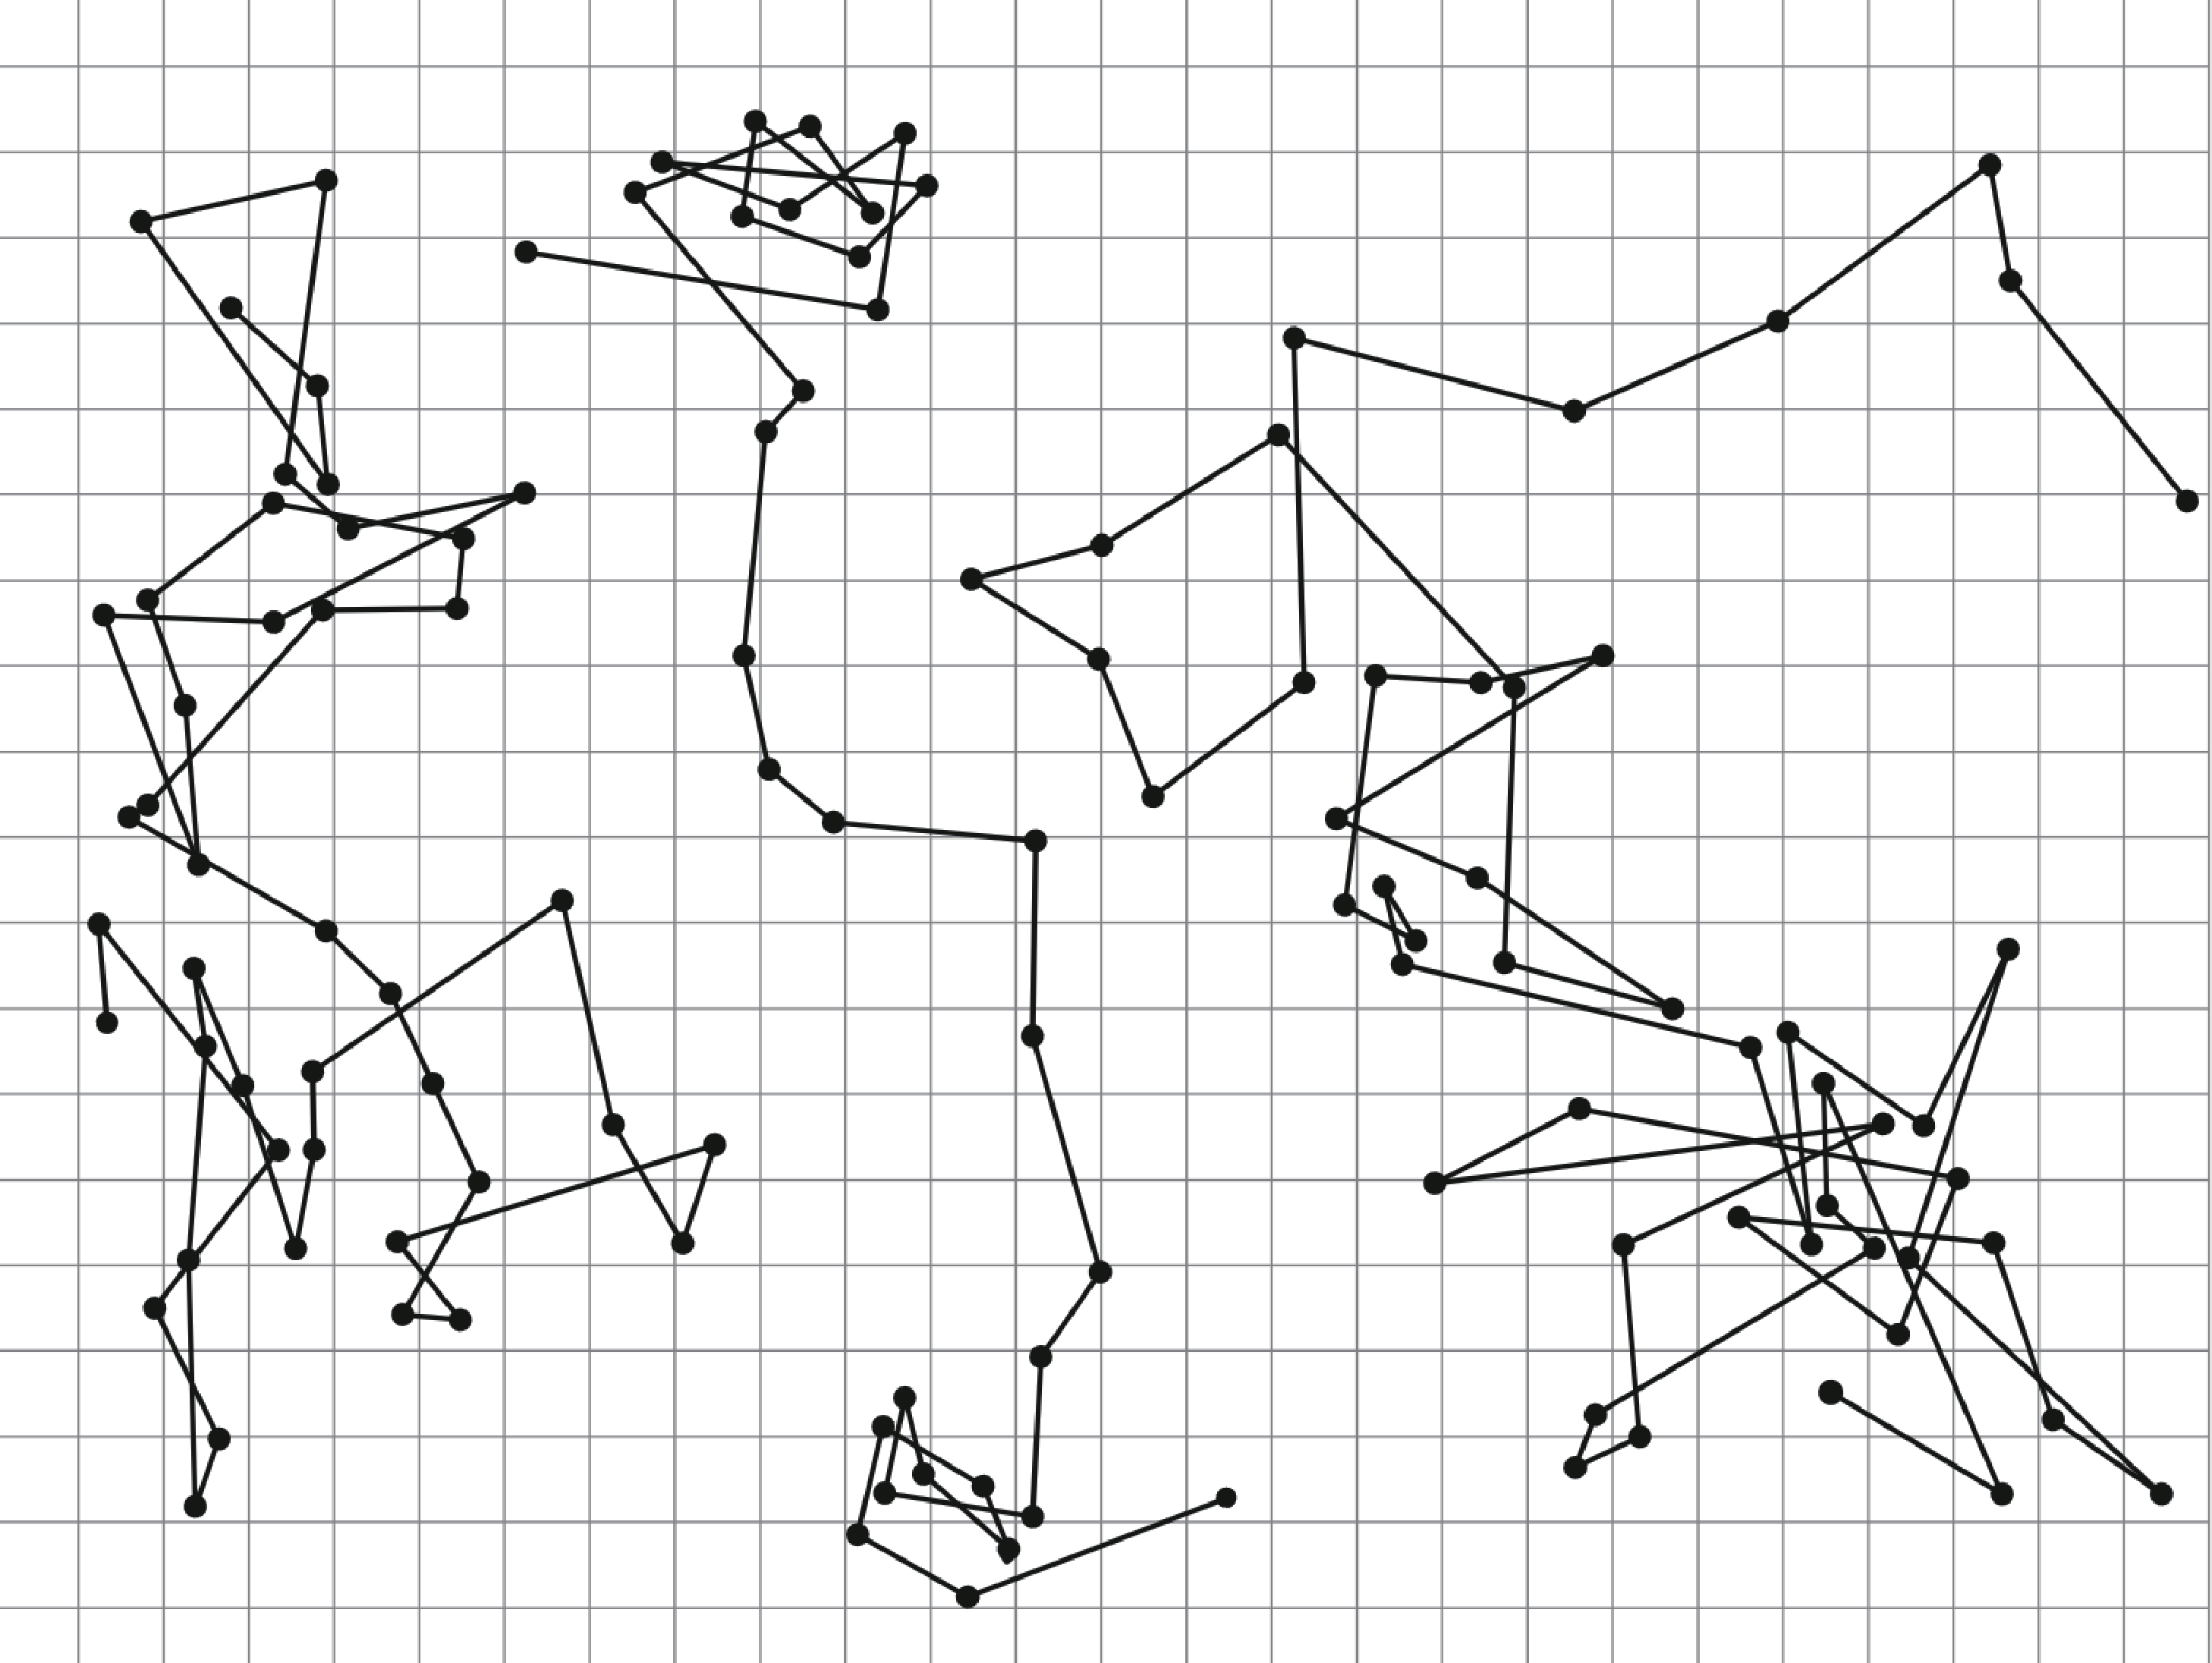
\includegraphics[width=6cm]{images/thermal-20.pdf}
 	\caption{记录到的分子运动轨迹}\label{fig: }
 \end{wrapfigure}
物理学家费曼(\textit{Richard P. Feynman})曾经有一段著名的论述:假如人类即将灭绝,你作为最后一个幸存者如果仅能够给未来的人类留下一条我们这个时代唯一一条科学知识的话,你会选择哪一个?
牛顿力学定律?爱因斯坦的相对论或者更近代的量子力学?对于这个问题不同的人有不同的答案,而费曼给出的则是{\heiti 原子假说}(atomic hypothesis)。

而{\heiti 分子动理论}(kenetic theory of molecules)告诉我们\CJKunderwave*{所有的物质都是由微小的、数目众多的微观颗粒所构成},不同物质的分子具有不同的空间分布,对于固体和液体来说分子之间的距离相对较小,某些固体分子还会有规则的空间排列,具有这种性质的物质称为晶体。所有的分子都做无规则的热运动,对于固体和液体来说,分子的热运动主要体现为在其原有位置附近的振动,而气体分子的运动范围相对较大,而且分子在运动过程中还可能发生碰撞。
单个分子的运动满足动力学定律,而物体的宏观性质则是由构成它的分子的微观性质所决定。在随后的学习过程中,我们需要特别关注的就是我们是如何通过对宏观物体性质的测量而推测它们的微观性质的,物体的宏观性质是如何由其微观组分以及它们的结构、运动所决定,不同的宏观性质之间是否可由微观属性给出其内在的联系。


在分子运动论的基础上,可以定性地分析一些复杂的物理过程,例如
\begin{example}
已知液体是由大量的分子构成,这些分子由于热运动而脱离液体的过程称之为蒸发,试从分子运动论的角度解析提高蒸发速度的三种方法:提高温度、增加液体表面面积以及提高液体表面空气流动的速度。
\tagged{student}{\vspace*{2cm}}
\begin{taggedblock}{teacher}
\newline
解析:温度反映了物体内分子做无规则运动的剧烈程度,温度越高,分子热运动越剧烈,所以蒸发越快;表面面积越大,分子跑出去的几率越大;
\end{taggedblock}
\end{example}


除了定性地分析,还可以通过微观性质定量地决定一些宏观的物理量
\begin{example}
NaCl晶体当中相邻的 Na 和 Cl 原子核之间的距离为 283 pm。
两种的相对原子质量分别为$35.45$, $22.99$,根据这些数据估算 NaCl 晶体的密度,并与实验值相比较。
\tagged{student}{\vspace*{3cm}}
\begin{taggedblock}{teacher}
\newline
解析:边长为相邻的 Na 和 Cl 原子核之间的距离的立方体体积为$283^3$,内含一个平均相对原子质量为29.22的原子,密度为$\frac{29.22m_0}{283^3}=2.148g/m^3$,实验值是$2.165g/cm^3$
\end{taggedblock}
\end{example}

由于分子之间的碰撞或相互作用,一般来说能量较大的分子会将能量传递给能量较小的分子。
这样经过一段时间以后分子之间通过相互作用经过充分的能量交换,使得每个分子的能量趋于相同。
当一个物体达到了这样的状态我们就称它处于{\heiti 热平衡}(thermal equilibrium)。
虽然从微观上看处于热平衡状态的物体的分子依然在做无规则的热运动,分子之间也会不断地碰撞,但对于每一个分子来说它从其它分子上获得的能量和传递给其它分子的能量一样多,这样从宏观上看物体的热性质就不再发生变化。
处于热平衡状态的物体每个分子每个自由度的平均能量都相同。
对于处于热平衡的物体,宏观上能够定义该物体的{\heiti 温度}(temperature)。
平衡时每个分子每个自由度上的平均能量越大的系统比起那些平均能量小的系统具有更高的温度,当把这两个物体相互接触时,由于分子之间的相互作用,那些具有较大平均能量的分子它们的能量就会传递给具有较小分子平均能量的物体。
从宏观上看,对应的过程就是热量由高温物体流向低温的物体。
在经典物理学中处于\CJKunderwave*{热平衡状态物体每个分子每个自由度上的平均能量和温度成线性关系},处于温度为$T$的物体分子每个运动自由度的平均能量为
\begin{equation}
\overline{E} = \frac{1}{2}kT,
\end{equation}
其中$k$称作玻尔兹曼({\textit Ludwig E. Boltzmann})常数
\begin{equation}\label{eqn: thermol-boltzmann-const}
k = \num{1.38064852(79)e-23}\si{J/K}.
\end{equation}
从上式可以清楚地看出玻尔兹曼常数给出了一个宏观物理量(温度)与微观物理量(平均能量)之间的关系,从这个意义上它是一个联系宏观和微观物理的桥梁,将来我们会知道它是所有包含统计观点物理定律中最重要的基本常数;
$T$为绝对温度,它和生活中常用的摄氏温度有着相同的间隔但不同的零点:
\begin{equation}\label{key}
T(\si{K}) = t(\si{^\circ C})+273.15,
\end{equation}
其中$t$为生活中常用的摄氏温度,$T$为热力学中的绝对温标。
它由对气体性质的研究中所发现并最终发现它的普适意义,实践上将纯水三相点的温度定义为$273.16\si{K}$。








\section{理想气体的性质}
\subsection{理想气体状态方程}
与固体或液体相比,气体分子之间的平均距离与它们本身的大小相比要大得多,与此同时分子之间的相互作用力也很弱。
如果气体足够稀薄可以认为分子的体积与气体所占据空间的体积相比忽略不计,分子之间的作用力也不与考虑,称具有这样性质的气体为{\heiti 理想气体}(ideal gas)。

密闭在一个给定大小容器当中的理想气体的状态由容器的体积$V$、气体对容器壁单位面积上的压力,也就是气体的压强$p$,和气体的温度所给出。
当气体的状态发生变化时,可以通过实验来确定描写气体状态的各个物理量的变化关系。
历史上理想气体的状态变化由三个著名的实验来给出:
\begin{description}
\item[{\heiti 玻意尔-马略特定律}(\textit{Boyle-Mariotte's Law})] \quad \par 温度保持不变的等温过程中,理想气体的压强和体积成反比: $pV = C$
\item[{\heiti 盖-吕萨克定律}(\textit{Gay-Lussac's Law})] \quad \par 体积保持不变的等容过程中,理想气体的压强和温度成正比:$p/T=C$
\item[{\heiti 查理定律}(\textit{Charles' Law})] \quad \par 压强保持不变的等压过程中,理想气体的体积与温度成正比:$V/T=C$
\end{description}


\quad\par
关于理想气体的三个实验定律可以统一总结为对于数量保持不变的理想气体在状态变化过程中
\begin{equation}
\frac{pV}{T}=const
\end{equation}
从中可以看出,对于同种数量的理想气体当它的压强、体积与温度三个量当中有两个量为已知时,另外一个物理量就被唯一确定。
对于不数量不同的理想气体,上式右边的常数不尽相同,随后可以证明该常数正比于气体的摩尔数$\nu$,这样上式可以写成
\begin{equation}\label{eqn: thermol 理想气体状态方程}
pV = \nu RT
\end{equation}
称为{\heiti 理想气体的状态方程}(State Equation of Ideal Gas),其中$\nu$为气体的摩尔数,$R$称为理想气体常数,它的近似值为
\begin{equation}\label{key}
R = 8.314\si{J/mol \cdot K}.
\end{equation}

%%%%%%%%%%%%%
\begin{example}
	根据理想气体状态方程完成下列问题:
	
	(1)体积增加的气体如果温度升高,则其压强将\kong\kong。
	
	(2)温度和压强均相同的气体体积之比等于其\kong\kong 之比。
	
	(3)相同数量的理想气体经过某一过程,压强变为原先的2倍,体积变为原先的2倍,这时温度变为原先的\kong 倍。
	
	
	\tagged{student}{\vspace*{4cm}}
	\begin{taggedblock}{teacher}
		\noindent
		解析:(1)增加。(2)气体摩尔数相比。(3)4
	\end{taggedblock}
\end{example}
%%%%%%%%%%%%%%%%%%%%



%%%%%%%%%%%%%
\begin{example}
	有一水银气压计,因水银柱上的玻璃管内有微量的空气,致使读数不准确。
	当大气压力为76~cmHg
	时,此气压计读数为74cm,此时其上空气柱长为8.0cm。若气压计读数为72.0cm时,则正确的 压力为多少?(不考虑温度变化)
	\tagged{student}{\vspace*{4cm}}
	\begin{taggedblock}{teacher}
		\newline
		解析:74.5cmHg
	\end{taggedblock}
\end{example}
%%%%%%%%%%%%%%%%%%%%

%%%%%%%%%%%%%
\begin{example}
	3.一根内径均匀、两端开口的细长玻璃管,竖直插在水中,管的一部分在水面上.现用手指封住管的上端,把一定量的空气密封在玻璃管中,以$ V_0$表示其体积;然后把玻璃管沿竖直方向提出水面,设此时封在玻璃管中的气体体积为$ V_1$;最后把玻璃管在竖直平面内转过$ 90^\circ$,使玻璃管处于水平位置,设此时封在玻璃管中的气体体积为$V_2$。则有
	
	$A. V_1>V_0=V_2,\qquad B. V_1>V_0>V_2,\qquad C.V_1=V_2>V_0,\qquad D, V_1>V_0,V_2>V_0$
	\tagged{student}{\vspace*{4cm}}
	\begin{taggedblock}{teacher}
		\noindent
		解析:A
	\end{taggedblock}
\end{example}
%%%%%%%%%%%%%%%%%%%%


%%%%%%%%%%%%%
\begin{example}
	如图所示,水平放置的汽缸内壁光滑,活塞厚度不计,在A、B 两处设有限制装置,使活塞只能在A、B之间运动,B左面汽缸的容积为$V_0$,A、 B之间的容积为$ 0.1V_0$。开始时活塞在 B处,缸内气体的压强为$ 0.9p_0$($p_0$为大气压强),温度为297K,现缓慢加热汽缸内气体,直至399.3K。
	
	(1)活塞刚离开B处时的温度$ T_B$; 
	
	(2)缸内气体最后的压强$ p$; 
	
	(3)在右图中画出整个过程的$ p-V$图像。
	
	\begin{center}
		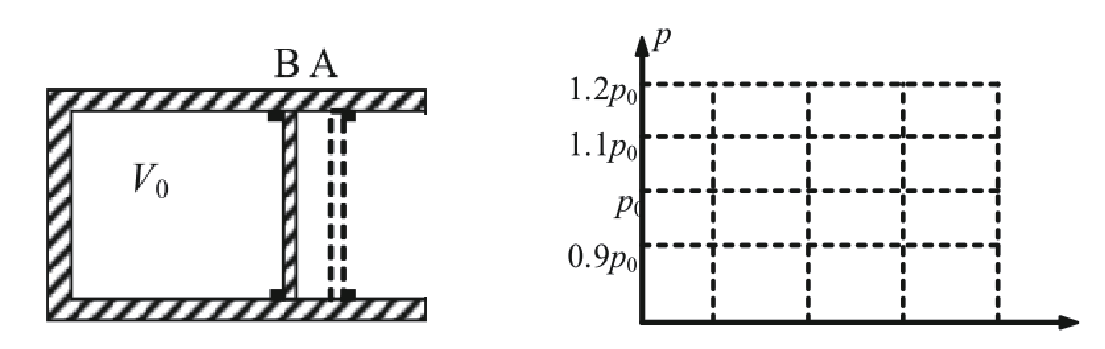
\includegraphics[width=0.6\linewidth]{images/thermal-1.pdf}
	\end{center}
	\tagged{student}{\vspace*{4cm}}
	\begin{taggedblock}{teacher}
		\noindent
		解析:(1)$T_B=330K$    (2)$p=1.1p_0$    (3)略
	\end{taggedblock}
\end{example}
%%%%%%%%%%%%%%%%%%%%


%%%%%%%%%%%%%
\begin{example}
	一个质量可不计的活塞将一定量的理想气体封闭在上端开口的直立圆筒形气缸内,活塞上堆放着铁砂,如图所示、最初活塞搁置在气缸内壁的固定卡环上,气体柱的高度为$ H_0$,压强等于大气压强$ p$。
	现对气体缓慢加热,当气体温度升高了$\Delta T=60K $时,活塞(及铁砂)开始离开卡环而上升、继续加热直到气柱高度为$ H_1=1.5H_0$、此后,在维持温度不变的条件下逐渐取走铁砂,直到铁砂全部取走时, 气柱高度变为$H_2=1.8H_0$,求此时气体的温度(不计活塞与气缸之间的摩擦)
		\begin{flushright}
			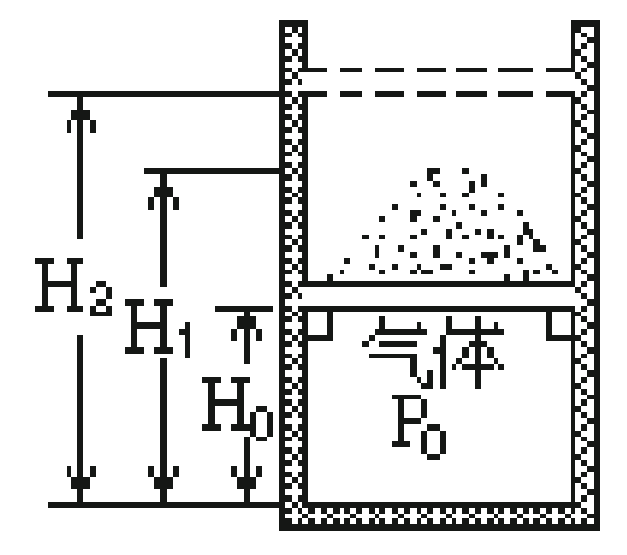
\includegraphics[width = 0.4\textwidth]{images/thermal-2.pdf} 
		\end{flushright}
	\tagged{student}{\vspace*{1cm}}
	\begin{taggedblock}{teacher}
		\noindent
		解析:540K
	\end{taggedblock}
\end{example}
%%%%%%%%%%%%%%%%%%%%


%%%%%%%%%%%%%
\begin{example}
	如图,在大气中有一水平放置的固定圆筒,它由$ a$、$b$ 和$ c$ 三个粗细不同的部分连接而成的,各部分的横截面积分别为$ 2S$ 、$\frac{1}{2} S $和$S$ 。已知大气压强为$p_0$,温度为$T_0$。
	两活塞$A$和$B$用一根长
	为$4l$的不可伸长的轻线相连,把温度为$T_0$的空气密封在两活塞之间,此时两活塞的位置如图所示。现对被密封的气体加热,使其温度缓慢上长升到$T$。若活塞与圆筒壁之间的摩擦可忽略,此时两活塞之间气体的压强可能为多少?
		\begin{flushright}
			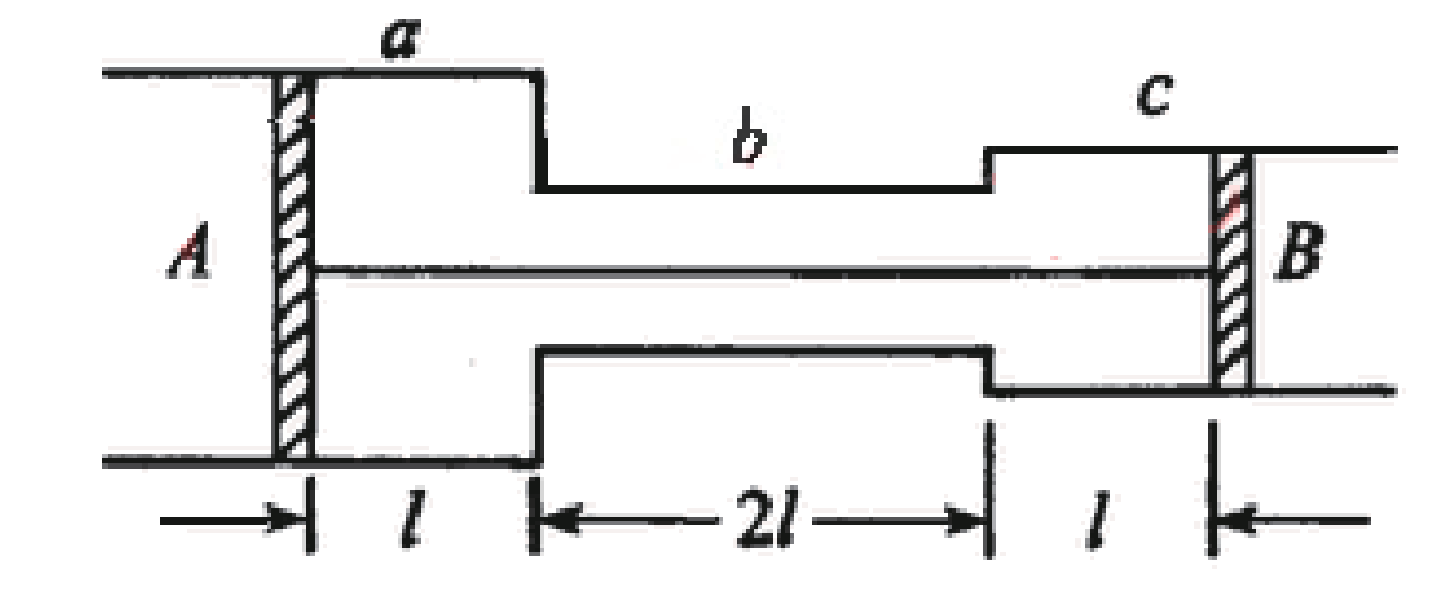
\includegraphics[width = 0.5\textwidth]{images/thermal-3.pdf} 
		\end{flushright}
	\tagged{student}{\vspace*{2cm}}
	\begin{taggedblock}{teacher}
		\noindent
		解析:两种情况:(1)$T\leq\frac{5}{4}T_0$时$p=p_0$     (2)$T>\frac{5}{4}T_0$时$p=\frac{4T}{5T_0}$
	\end{taggedblock}
\end{example}
%%%%%%%%%%%%%%%%%%%%


%%%%%%%%%%%%%
\begin{example}
	如图所示,竖直放置的圆柱形气缸固定不动,A、B两活塞的面积分别为 $S_A=20 cm^2$,$S_B=10 cm^2,$ 它们用一根轻绳连接,B 又与另一根竖直轻绳相连,绳跨过两定滑轮与重物 C 相接,已知 A、B 两活塞的质量$m_A=2m _B=1 k\si{kg}$,活塞静止时,气缸中理想气体压强$ p_1=1.2 atm$,温度为 $T_1=800 \si{K}$, 上、下气柱长分别为$ 2L $及$ L$,不计摩擦,且大气压强为标准大气压,上气缸足够长,求:
	(1)重物C的质量$M$, (2)缓慢降低气缸内气体的温度直至$ 210 K$,试在 $p-V$图上画出缸内气体状态变化的图线,并计算出图线拐点处气体的温度及最终 B活塞位置。 (1atm取 $10^5\si{Pa}$)。
		\begin{flushright}
			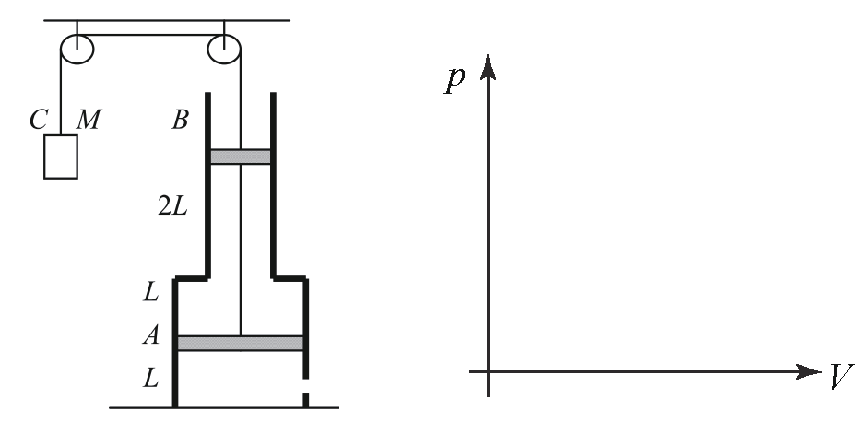
\includegraphics[width = 0.5\textwidth]{images/thermal-4.pdf} 
		\end{flushright}
	\tagged{student}{\vspace*{3cm}}
	\begin{taggedblock}{teacher}
		\noindent
		解析:(1)$M=2kg$      (2)略
	\end{taggedblock}
\end{example}
%%%%%%%%%%%%%%%%%%%%


%%%%%%%%%%%%%
\begin{example}
	如图所示,开口向上粗细均匀的玻璃管长$L = 100\si{cm}$,管内有一段高$h=20\si{cm}$的水银柱,封闭着长$a=50\si{cm}$的空气柱,大气压强$p_0 = 76\text{cmHg}$,温度$t_0 \ 27\si{\degreeCelsius}$,求温度更少升到多高时可使水银全部溢出?
		\begin{flushright}
			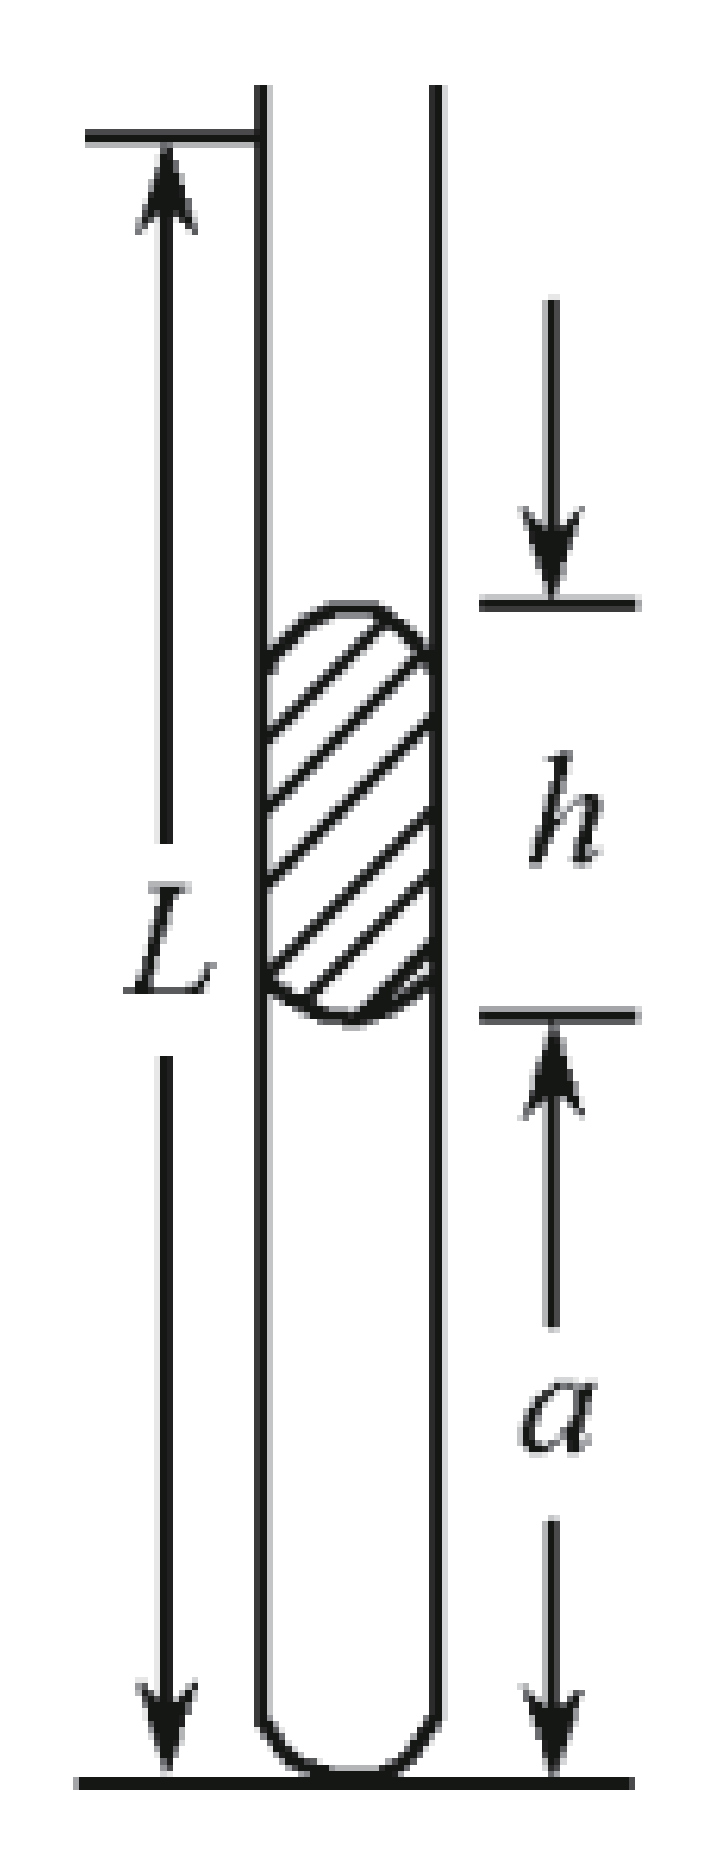
\includegraphics[width = 0.1\textwidth]{images/thermal-9.pdf} 
		\end{flushright}
	\tagged{student}{\vspace*{1cm}}
	\begin{taggedblock}{teacher}
		\noindent
		解析:484K
	\end{taggedblock}
\end{example}
%%%%%%%%%%%%%%%%%%%%

%%%%%%%%%%%%%
\begin{example}
	一根长为$ L($以厘米为单位)的粗细均匀的、可弯曲的细管,一端封闭,
	一端开口,处在大气中。大气的压强与$H$厘米高的水银柱产生的压强相等,已知管长$ L>H$。 现把细管弯成 L形,如图所示,假定细管被弯曲时,管长和管的内径都不发生变化。可以把水银从管口徐徐注入细管而不让细管中的气体泄出。
	当细管弯成 L形时,以$ l $表示其竖直 段的长度,问$ l $取值满足什么条件时,注入细管的水银量为最大值?
	给出你的论证并求出水银量的最大值(用水银柱的长度表示)。
		\begin{flushright}
			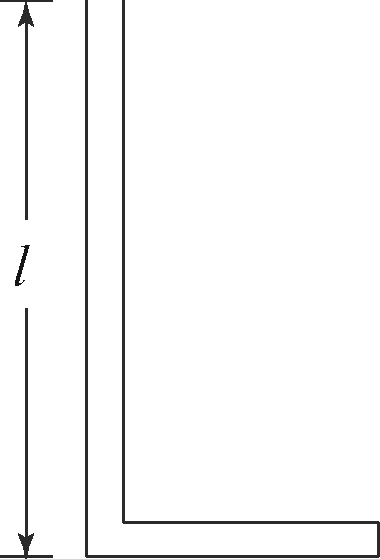
\includegraphics[width = 0.2\textwidth]{images/thermal-5.pdf} 
		\end{flushright}
	\tagged{student}{\vspace*{3cm}}
	\begin{taggedblock}{teacher}
		\noindent
		解析:$l≥L-H$时,注入的水银柱的长度x的最大值$x_{max}=L-H$
	\end{taggedblock}
\end{example}
%%%%%%%%%%%%%%%%%%%%

\subsection{理想气体状态方程的微观解释}
大量气体分子与容器壁持续不断的碰撞从宏观上看就表现为气体的压力,根据定义单位面积上的压力就是气体{\heiti 压强}(pressure)。
为简单起见假设容积为$V$的容器当中只包含有同种气体,每个气体分子的质量为$m$,总共有$N$个分子。
考虑容器内部一个面积为$S$,垂直于$x$轴的给定的区域,如果一个气体分子速度的$x$分量为$v_x$与器壁发生完全弹性碰撞,该分子的$x$方向上的动量改变量为
\begin{equation}
\Delta p_x = 2mv_x,
\end{equation}
对于给定的时间间隔$\dt$当中,能够发生这样碰撞的几率则是底面积为$S$,高为$v_x\dt$的圆柱体面积与容器容积$V$之比$Sv_x\dt/V$,这样在$\dt$时间里那些能够与器壁发生碰撞的分子总的动量的改变量就是
\begin{equation}
\Delta p_x = \frac{1}{2}\sum_{i=i}^N\left(2mv_{ix}\right)\left(\frac{Sv_{ix}\dt}{V}\right) = \frac{mS\dt}{V}\sum_{i=i}^Nv_{ix}^2,
\end{equation}
其中$v_{ix}$为编号为$i$的分子速度的$x$分量,上式第二项求和号外部的$\frac{1}{2}$因子是由于前面的统计方式当中除了包含向着器壁运动的分子以外那些以相同的速度背着器壁方向运动的分子也被包含了进来,由于处于热平衡的气体的运动是杂乱无章的,两种速度运动的分子可以认为各占一半。
气体分子速度的变化是由器壁对分子的作用力所导致,根据牛顿第三定律气体分子也会对器壁有相等大小的作用力,简单的数学推导可以得出气体压强为
\begin{equation}
p = \frac{F}{S} = \frac{m}{V}\sum_{i=i}^Nv_{ix}^2 = \frac{mN}{V}\left(\frac{1}{N}\sum_{i=i}^Nv_{ix}^2\right) = nm\overline{v_x^2}
\end{equation}
其中$\overline{v_x^2}$代表分子速度的$x$分量的平方的平均值,$n=N/V$为分子的数密度,即单位体积内的气体分子数。

处于热平衡的气体分子运动是各向同性的,具有性质$\overline{v_x^2}=\overline{v_y^2}=\overline{v_z^2}=\frac{1}{3}\overline{v^2}$,这样气体的压强又可以写为
\begin{equation}
p = \frac{2}{3}n\overline{\left(\frac{1}{2}mv^2\right)} = \frac{2}{3}n\overline{\epsilon_k} = \frac{2}{3}u,
\end{equation}
其中$u$为单位体积内气体分子的平均平动动能。
从中可以看出理想气体的压强正比于分子数密度和每个分子的平均平动动能。
由于气体分子的平动共有三个自由度,根据能量均分可知平均平动动能$\overline{\epsilon_k}=\frac{3}{2}kT$,将这个结论代入压强的表达式并做恒等变形可得
\begin{equation}
p = nkT \qquad;\qquad pV = NkT = \frac{N}{N_A}N_AkT = \nu RT
\end{equation}
其中$N_A$为阿伏伽德罗常数,$N/N_A$恰为气体的摩尔数$\nu$,将上式与理想气体的状态方程\ref{eqn: thermol 理想气体状态方程}相比较可以看出理想气体常数$R$就是由阿伏伽德罗常数和玻尔兹曼常数的乘积
\begin{equation}
R=N_A k= \num{8.3144598(48)}\si{J/mol \cdot K}.
\end{equation}

通过气体压强的微观机制还能够解释气体的一些其它性质
\begin{example}
气体的压强是由气体分子和容器壁的弹性碰撞所产生,在此基础上请说明:
\begin{enumerate}
\item 无论容器的形状如何,气体对于容器壁的压力总是垂直于容器的表面且等于压强与该处容器表面积的乘积。
\item  道尔顿分压定律:在任何容器内的气体混合物中,如果各组分之间不发生化学反应,则每一种气体都均匀地分布在整个容器内,它所产生的压强和它单独占有整个容器时所产生的压强相同。
\item 混合气体的状态方程: 如果一个容器内有$N$种理想气体,每种气体的摩尔数分别为$\nu_i$,它们处于热平衡状态,这样气体的状态方程为
\begin{equation}
pV = \left(\sum_{i=1}^N \nu_i\right)RT
\end{equation}
\end{enumerate}
\tagged{student}{\vspace*{4cm}}
\begin{taggedblock}{teacher}
\noindent
解析:1. 从微观的弹性碰撞过程可以看出,无论容器壁的形状为何,气体分子反弹所产生对器壁的冲量均沿着法线方向,可以说明压强的方向。

2. 不同气体分子的碰撞“看上去”与每种气体分子单独存在产生的冲量一样大,但是要注意当把多种气体放在一起时其实它们之间也会发生碰撞导致本应当撞向器壁的那些分子由于碰到另外的分子而撞不上去。
所以更准确地说分压定律仅在理想气体,即气体足够稀薄的情况下才能够由微观机制给出。

3. 在分压定律的基础上很容易证明这一点,不解释。
\end{taggedblock}
\end{example}

\begin{example}
一个容积为$V$的容器被一个挡板分为体积相等的两部分,左半部分中装有压强为$p$温度为$T$的理想气体,右半部分为真空。
现将挡板突然抽出,气体将向真空扩散,求在气体再次达到平衡状态时的温度和压强。
\tagged{student}{\vspace*{4cm}}
\begin{taggedblock}{teacher}
\newline
解析:$T'=T, p'=\frac{1}{2}p$
\end{taggedblock}
\end{example}



\subsection{气体的内能}
在静止容器当中处于平衡状态的气体虽然没有宏观的整体运动,但是由于每个分子都具在作热运动所以此时气体依然包含有一定的能量,物体的{\heiti 内能}(internal energy)被定义为构成物体分子的动能,分子内势能和分子之间势能的总和。
对于理想气体来说由于分子之间的作用力被忽略不计,所以分子之间没有势能,而分子内部也没有发生任何改变(化学反应),所以分子内势能也不变,这样理想气体的内能就是分子动能和总和\footnote{改变势能零点取分子内势能为零},它与温度有密切的关系,但理想气体的体积不会影响内能。


向处于容积不变的密闭容器当中的气体输送给定的热量,根据能量守恒热量全部变成气体的内能。
此时输入的热量与气体温度的改变量称做气体的{\heiti 等容热容量}(heat capacity at constant volumn),记做$C_V$:
\begin{equation}
C_v = \frac{\Delta Q}{\Delta T},
\end{equation}
对于理想气体来说内能与体积无关,只和温度有关,当温度上升$\Delta T$时内能的改变量为
\begin{equation}
\Delta U = C_v\Delta T.
\end{equation}
给定数量理想气体的等容热容量与其摩尔数成简单的正比关系,我们将每摩尔气体的等容热容量称为{\heiti 摩尔定容热容量}(molar heat capacity at constant volumn),通常用$c_V$来表示,这样我们有$C_V = \nu c_V$。

对于单原子分子的理想气体(氦气、氖气),当处于温度为$T$的平衡状态时每个分子的平均动能$\overline{\epsilon_k}=\frac{3}{2}kT$。
这样$n$摩尔单原子分子气体的内能无论体积如何均为
\begin{equation}
U = N\cdot \frac{3}{2}kT = \frac{3}{2}\frac{N}{N_A}N_AkT = \frac{3}{2}\nu RT.
\end{equation}
实际测量的结果与理论预测非常接近。
并且可知单原子气体的摩尔等容热容量$c_V = \frac{3}{2}R$。

多原子分子理想气体的内能则较为复杂。
实验表明在室温$T\sim 300\unit{K}$附近,双原子分子气体(例如氢气、氧气、氮气、氯气为双原子分子)等容摩尔比热大约为$c_V\sim\frac{5}{2}R$,随着温度的增加$c_V$会缓慢增加,当温度达到$2000\unit{K}$左右时$c_V\sim\frac{7}{2}R$。
这其中的原理只有当我们学习了量子力学以后才能了解,对于我们现阶段来说题目当中一定会告诉我们当中气体的内能准确的表达式。


\begin{figure}[h]
	\centering
	\includegraphics[width=0.5\linewidth]{images/before-th-1}
	\caption{气体对外做功为$p-V$图中过程曲线与横轴包围的面积}
	\label{fig:before-th-1}
\end{figure}


\subsection{气体的作功}
当气体的体积发生变化时会向外作{\heiti 功}(work),反之当气体被压缩时必须有外力抵抗气体压力向气体作功。
等容变化的气体由于体积不变所以没有作功。
等压过程的功的计算较为简单,可以证明当气体膨胀时向外做功就是压强和体积变化量的乘积:
\begin{equation}
W=p\Delta V,
\end{equation}
其中$\Delta V$为一个过程前后体积的变化量,当气体体积增加时它将向外做正功,反之气体被压缩,这时外力将对气体做正功,相应地气体对外则做负功。


对于一般的气体过程气体所做的功没有办法以简单的方式进行计算。
通常我们只考虑那种气体状态经历缓慢变化的过程,在此过程中的每一个瞬间气体都可以近似地看做处于平衡状态,一般来说只要气体状态改变比较慢这个假设就被认为是成立的,这样的过程被称为{\heiti 准静态过程}(quasistatic process)。
一个普遍的结论是对于准静态过程,其状态变化可用$p-V$图中的一条曲线来描写,这时气体对外作功的大小等于曲线所围成的面积,当体积变大则向外作功,体积变小外界对气体做功。
例如体积为$V_1$的理想气体等温膨胀到$V_2$向外作功的大小等于等温曲线下的面积,数学上可以证明温度为$T$等温膨胀过程的功
\begin{equation}
W = \nu RT\ln \frac{V_2}{V_1}
\end{equation}
对于那些不是准静态过程气体的功不能够按照这样的方法计算,必须通过其它条件来确定。












\section{热力学第一定律}
\subsection{热力学中的能量转化与守恒}
\begin{wrapfigure}{r}{5cm}
	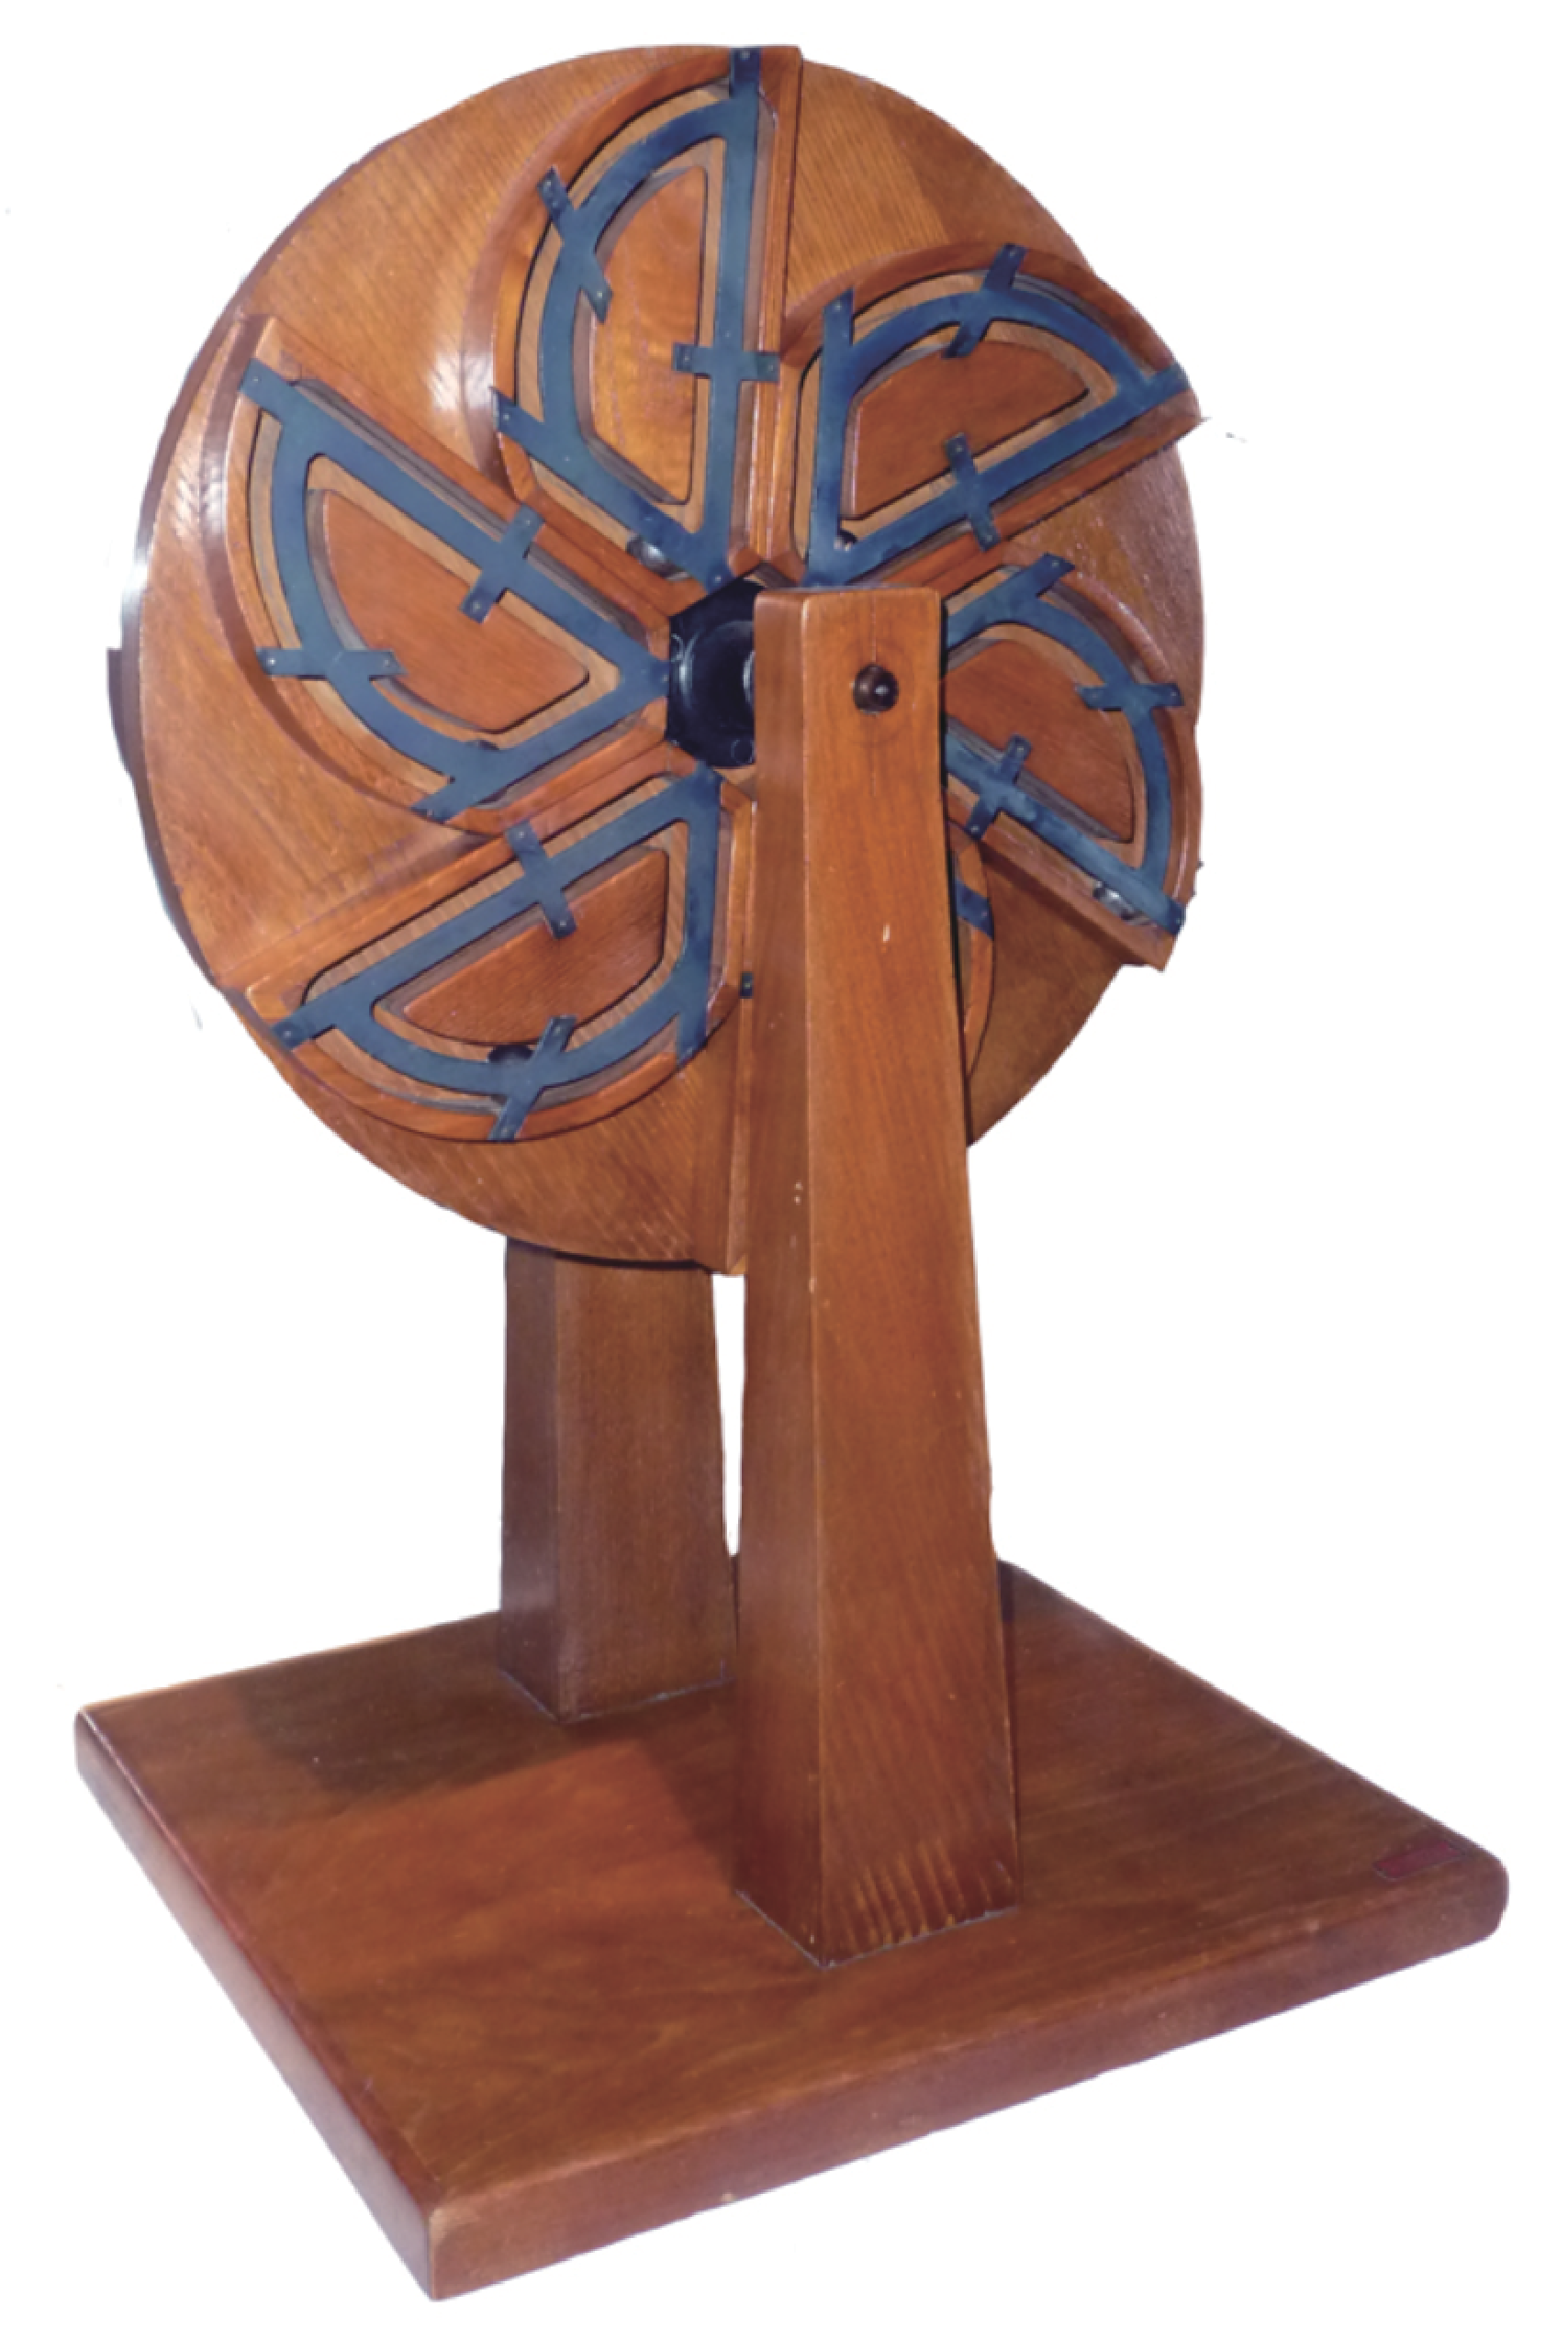
\includegraphics[width=5cm]{images/thermal-19.pdf} 
	\caption{假想的永动机模型}\label{fig: }
\end{wrapfigure}
在今天,能量的转化与守恒定律已经根深蒂固地存在于我们的脑海当中,在热力学中能量的转化和守恒定律体现为{\heiti 热力学第一定律}(first law of thermodynamics)。
热力学第一定律告诉我们,热量可以从一个物体传递到另一个物体,也可以与机械能或其他能量互相转换,但是\CJKunderwave*{在转换过程中,能量的总值保持不变}。对一个热力学系统所传递的热量(通过微观分子碰撞转移的能量),再加上对它所作的机械功(通过宏观分子的移动所转移的能量),最终全部被归结为该热力学系统内能的增量;同样热力学系统内能的降低最终必然表现为它向外界传递的热量以及可能的对外作功。
当热力学系统发生了一定的变化,如果用$Q$来表示该过程当中向一个热力学系统传递的热量,$W$代表对该系统所作的功,那么这个热力学系统内能的变化量$\Delta U$可以表示为
\begin{equation}\label{eqn: thermol 热力学第一定律}
\Delta U = Q+W.
\end{equation}


使用热力学第一定律的过程中应该注意以下几个问题:
\begin{enumerate}
\item 公式\ref{eqn: thermol 热力学第一定律}的右边第一项代表的是向该系统传递的热量,第二项为对其作的功。
在实际应用当中,热量和机械能的传递方向起着至关重要的作用,千万不要搞混。
\item 向一个系统传递热量的方式有很多,如摩擦生热、化学燃料燃烧、接触热传递、通电使电阻发热、辐射传热甚至通过原子核反应而产生热量等。
以不同的方式产生热量的大小由对应过程所满足的物理规律所决定。
\item 虽然热力学第一定律可以应用于各种热力学系统,现阶段我们主要关注气体状态变化的过程。
$n$摩尔理想气体内能的变化量由摩尔等容热容量和温度变化量共同决定:
\begin{equation}
\Delta U = \nu c_V\Delta T,
\end{equation}
其中$c_V$为其摩尔等容热容量,$\Delta T$为温度变化。
在状态变化过程中,气体的体积有时会发生变化,当体积有微小改变时\ref{eqn: thermol 热力学第一定律}当中的功为
\begin{equation}
\Delta W = -p\Delta V
\end{equation}
体积减小时外力对系统做正功,表达式中的$\Delta W$为正值。
\item 内能的变化量只与特定过程前后热力学系统的状态有关,与变化的方式无关;但热量和功却与状态改变的方式,即过程有关。
对于相同始末状态不同过程当中的热量和功可能不同,但对于所有过程内能的变化量却一致。
另外热力学第一定律不仅对于准静态过程成立,对于那些快速发生的过程同样成立,但要注意这时对气体做功不能够用$p-V$图中的面积来确定。
\end{enumerate}




%%%%%%%%%%%%%
\begin{example}
	压强为\num{1.0e5}\si{Pa},体积为\num{0.0082}\si{m^3}的氮气,从初始温度 300K加热到400K,对于体积不变和压强不变的加热过程,求各需要多少热量,哪一个过程所需要的热量大,为什么?
	\tagged{student}{\vspace*{4cm}}
	\begin{taggedblock}{teacher}
		\newline
		解析:压强不变需要的热量大,因为还需要对外做功。$Q_1=683J , Q_2=957J$
	\end{taggedblock}
\end{example}
%%%%%%%%%%%%%%%%%%%%


%%%%%%%%%%%%%
\begin{example}
如图所示,有一定量的单原子理想气体,从初态 $a(p_1,V_1)$开始经过一个等容过程达到状态$ b$,再经过一个等压过程来到状态$c$,最后经等温过程而完成一个循环,已知$ 1\si{mol}$该气体温度改变 1K 内能变化为$c_v = \frac{3}{2}R$,


1. 由$ c $到$ a $气体是吸热还是放热,具体吸放热多少? 
	
2. 由$ a $到$ b $气体是吸热还是放热,具体吸放热多少? 

3. 由$ b$ 到$ c $气体是吸热还是放热,具体吸放热多少? 

4. 整个循环过程净功多少,净吸放热多少?
	\begin{flushright}
		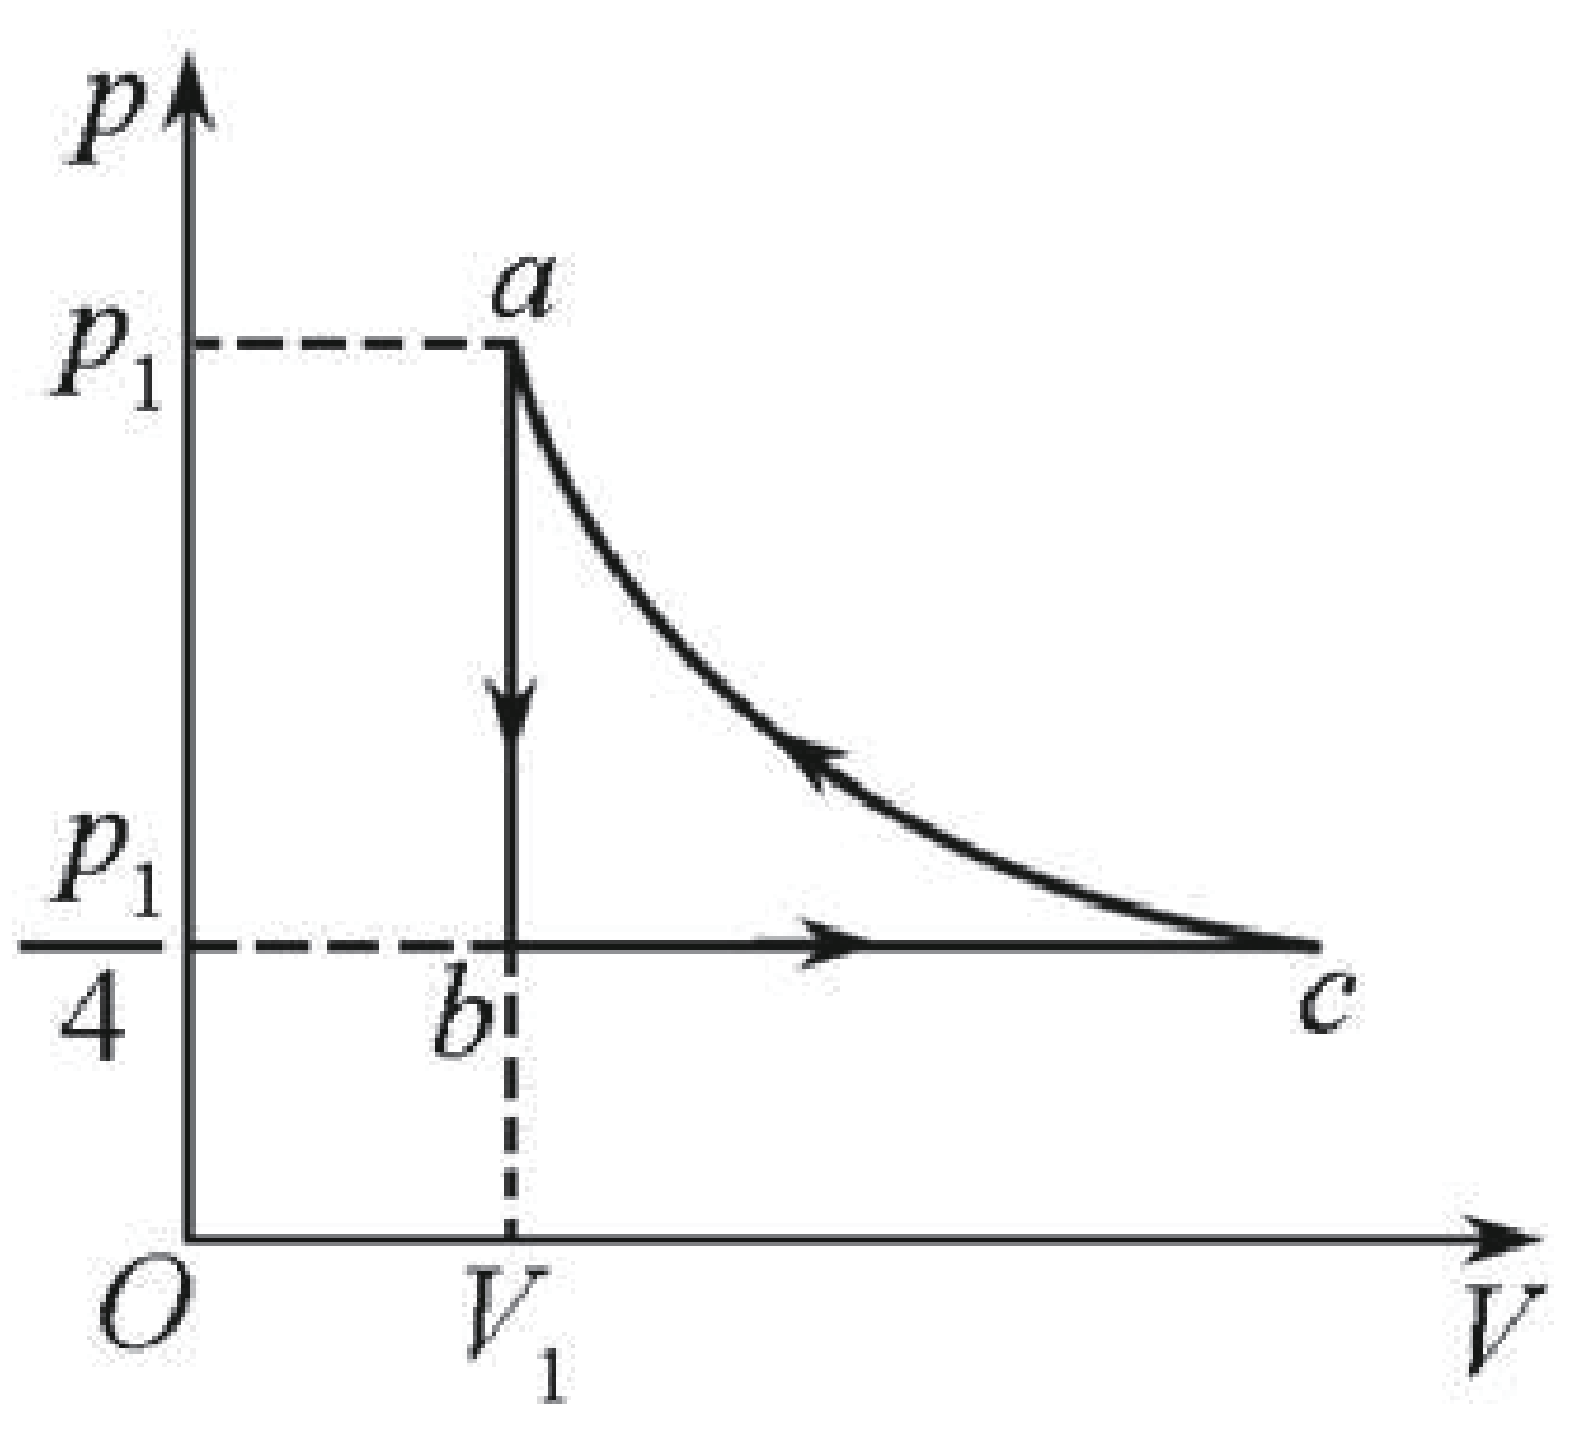
\includegraphics[width = 0.3\textwidth]{images/thermal-10.pdf} 
	\end{flushright}
	\tagged{student}{\vspace*{2cm}}
	\begin{taggedblock}{teacher}
		\noindent
		解析:1.放热,外界对气体做功 $Q_1=\ln4p_1V_1$
		\\2.放热,内能减少 $Q_2=\frac{9}{8}p_1V_1$
		\\3.吸热,对外界做功且内能增加 $Q_3=\frac{15}{8}p_1V_1$
		\\4.$W=\Delta Q=(\ln4-\frac{3}{4})p_1V_1$
	\end{taggedblock}
\end{example}
%%%%%%%%%%%%%%%%%%%%



%%%%%%%%%%%%%

\begin{example}
	一定质量的理想气体经历了$p-T$图线所示 ab、bc、cd、da 四个过程,其中 ab 垂直于OT,bc 的延长线经过O点,cd平行于OT,da 平行于 cb,由图可以判断( )
	
\begin{center}
	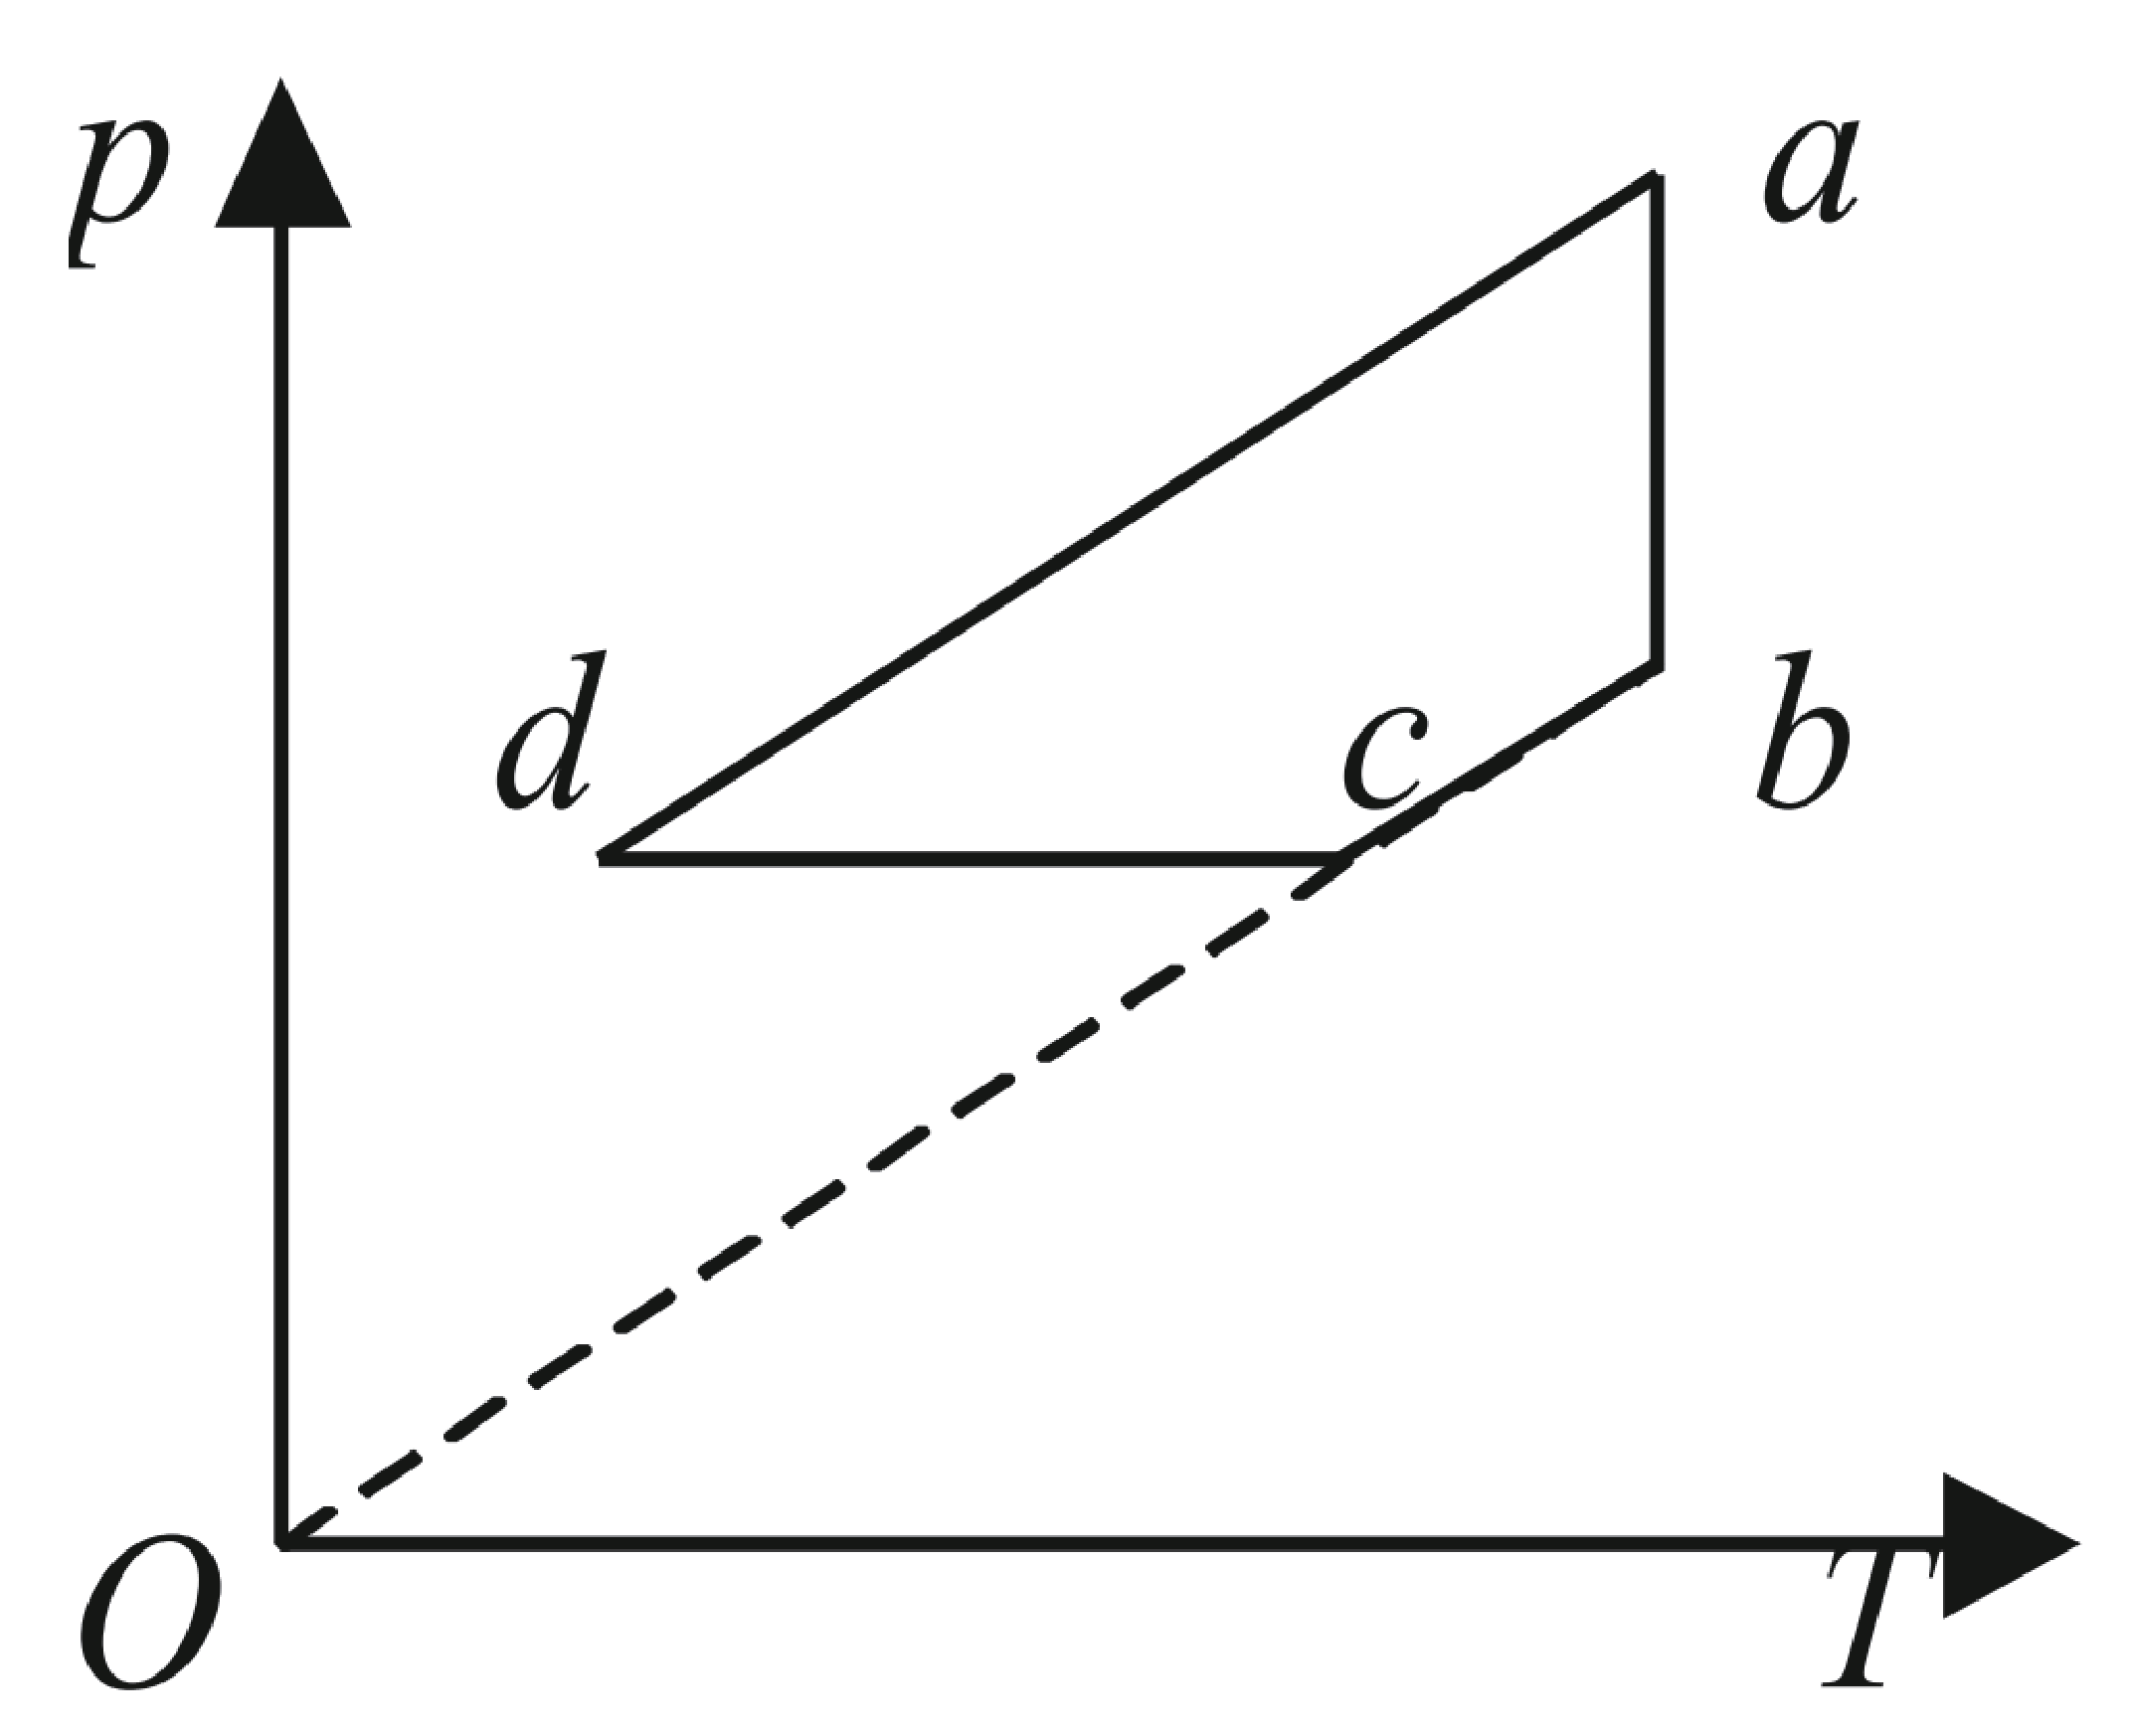
\includegraphics[width=5cm]{images/thermal-12.pdf} 
\end{center}
	 
	
	A.ab 过程中气体的体积增大,分子平均动能不变。
	
	 B.bc 过程中气体的体积增大,内能减小。
	 
	  C.cd过程中气体的体积减小,分子平均动能减小。
	  
	   D.da 过程中气体的体积增大,内能增大。

	\tagged{student}{\vspace*{0cm}}
	\begin{taggedblock}{teacher}
		\noindent
		解析:ACD
	\end{taggedblock}
\end{example}
%%%%%%%%%%%%%%%%%%%%

%%%%%%%%%%%%%
\begin{example}
如图所示,绝热的活塞$ S $把一定质量的稀薄气体(可视为理想气体)密封在水平放置的绝热气缸内。
活塞可在气缸内无摩擦地滑动,气缸左端的电热丝可通弱电流对气缸内气体十分缓慢地加热,气缸处在大气中,大气压强为$p_0$,初始时气体的体积为$V_0$,压强为$p_0$。
已知 1 摩尔该气体温度升高 1K 时其内能的增量为一已知恒量$ C$,求以下两种过程中电热丝传给气体的热量$Q_1$与$Q_2$之比。

1.从初始状态出发,保持活塞$ S $位置圈定,在电热丝中通以弱电流,并持续一段时间,然后停止通电,待气体达到热平衡时,测得气体的压强为$p_1$.
	
	2.仍从初始状态出发,让活塞处在自由状态,在电热丝中通过弱电流,也持续一段时间,然后停止通电,最后测得气体的体积为$V_2$.
	
		\begin{flushright}
			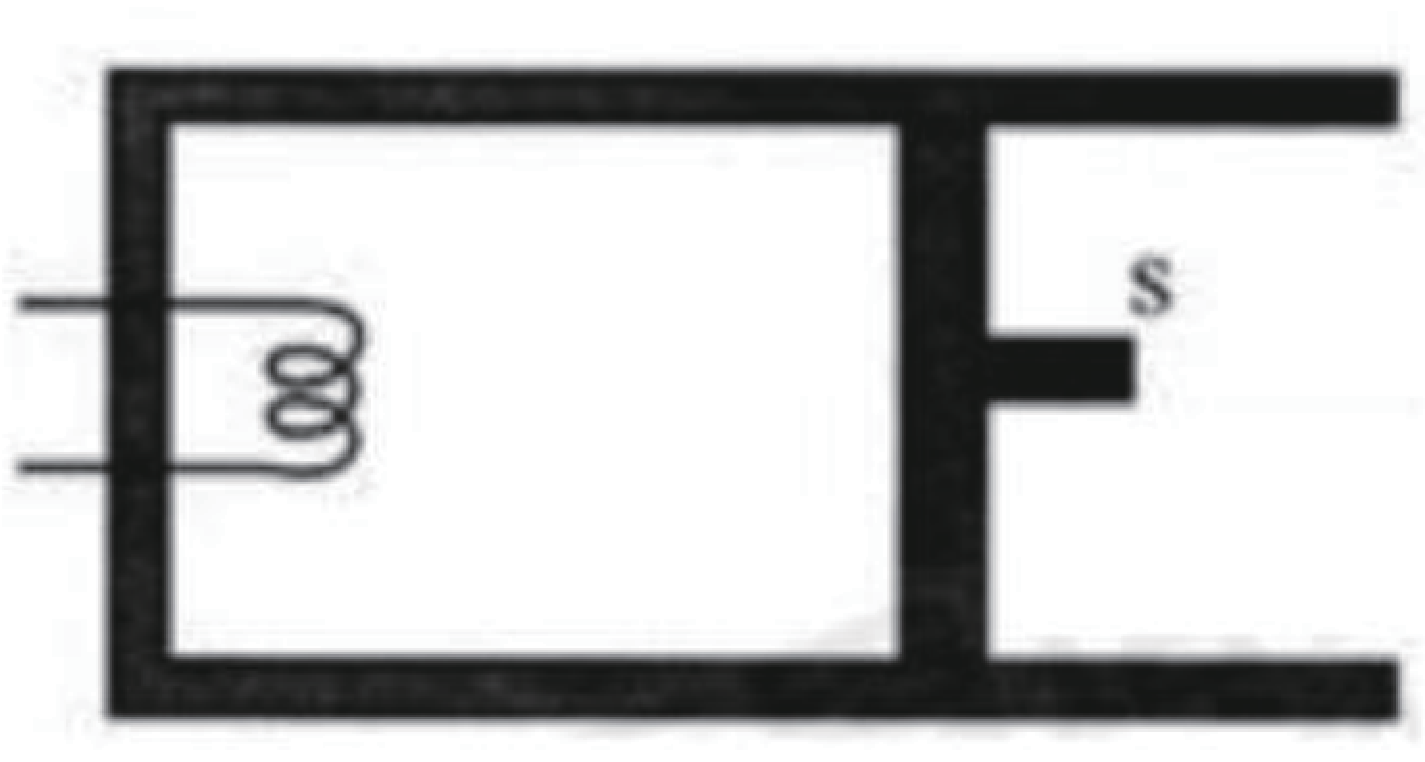
\includegraphics[width = 0.3\textwidth]{images/thermal-6.pdf} 
		\end{flushright}
	\tagged{student}{\vspace*{2cm}}
	\begin{taggedblock}{teacher}
		\noindent
		解析:1.$\frac{C}{R}(p_1-p_0)V_0$
		\\2.$\frac{C+R}{R}(V_2-V_0)p_0$
	\end{taggedblock}
\end{example}
%%%%%%%%%%%%%%%%%%%%


%%%%%%%%%%%%%
\begin{example}
	如图所示,一摩尔理想气体,$p-V$图中的状态$ A$出发,经过一缓慢地直线过程到达状态$ B$,已知状态$ B $的压强与状态$ A $的压强之比为$\frac{1}{2}$,若要使整个过程的最终结果是气体从外界吸收了热量,则状态$B $与状态$A $的体积之比应满足什么条件?
	已知此理想气体每摩尔的内能为$ \frac{3}{2}RT $,$R$为普适气体常量,$T$为热力学温度.
		\begin{flushright}
			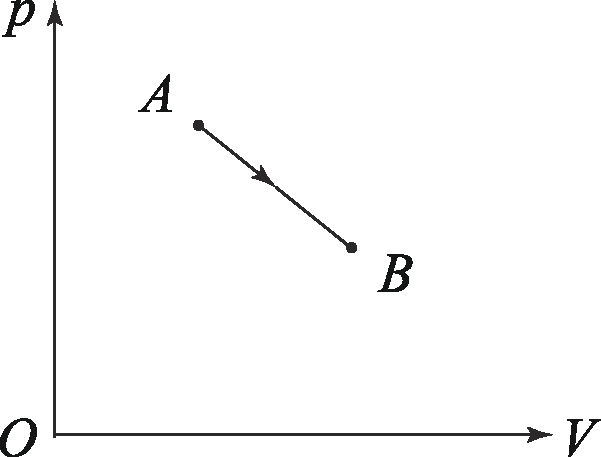
\includegraphics[width = 0.3\textwidth]{images/thermal-7.pdf} 
		\end{flushright}
	\tagged{student}{\vspace*{2cm}}
	\begin{taggedblock}{teacher}
		\noindent
		解析:$\frac{V_B}{V_A}>\frac{3}{2}$
	\end{taggedblock}
\end{example}
%%%%%%%%%%%%%%%%%%%%

%%%%%%%%%%%%%
\begin{example}
	$n\si{mol}$氧气由初态 A(体积$ V_1$)沿如图所示的直线路径变到末态 B (体积$V_2$),状态变化满足$p=kV$($k$为已知常数)。
	试求上述过程中,气体内能的变化量,对外界所作的功和从外界吸收的热量(设氧气可视为理想气体,且$c_v =\frac{5}{2}R$)
		\begin{flushright}
			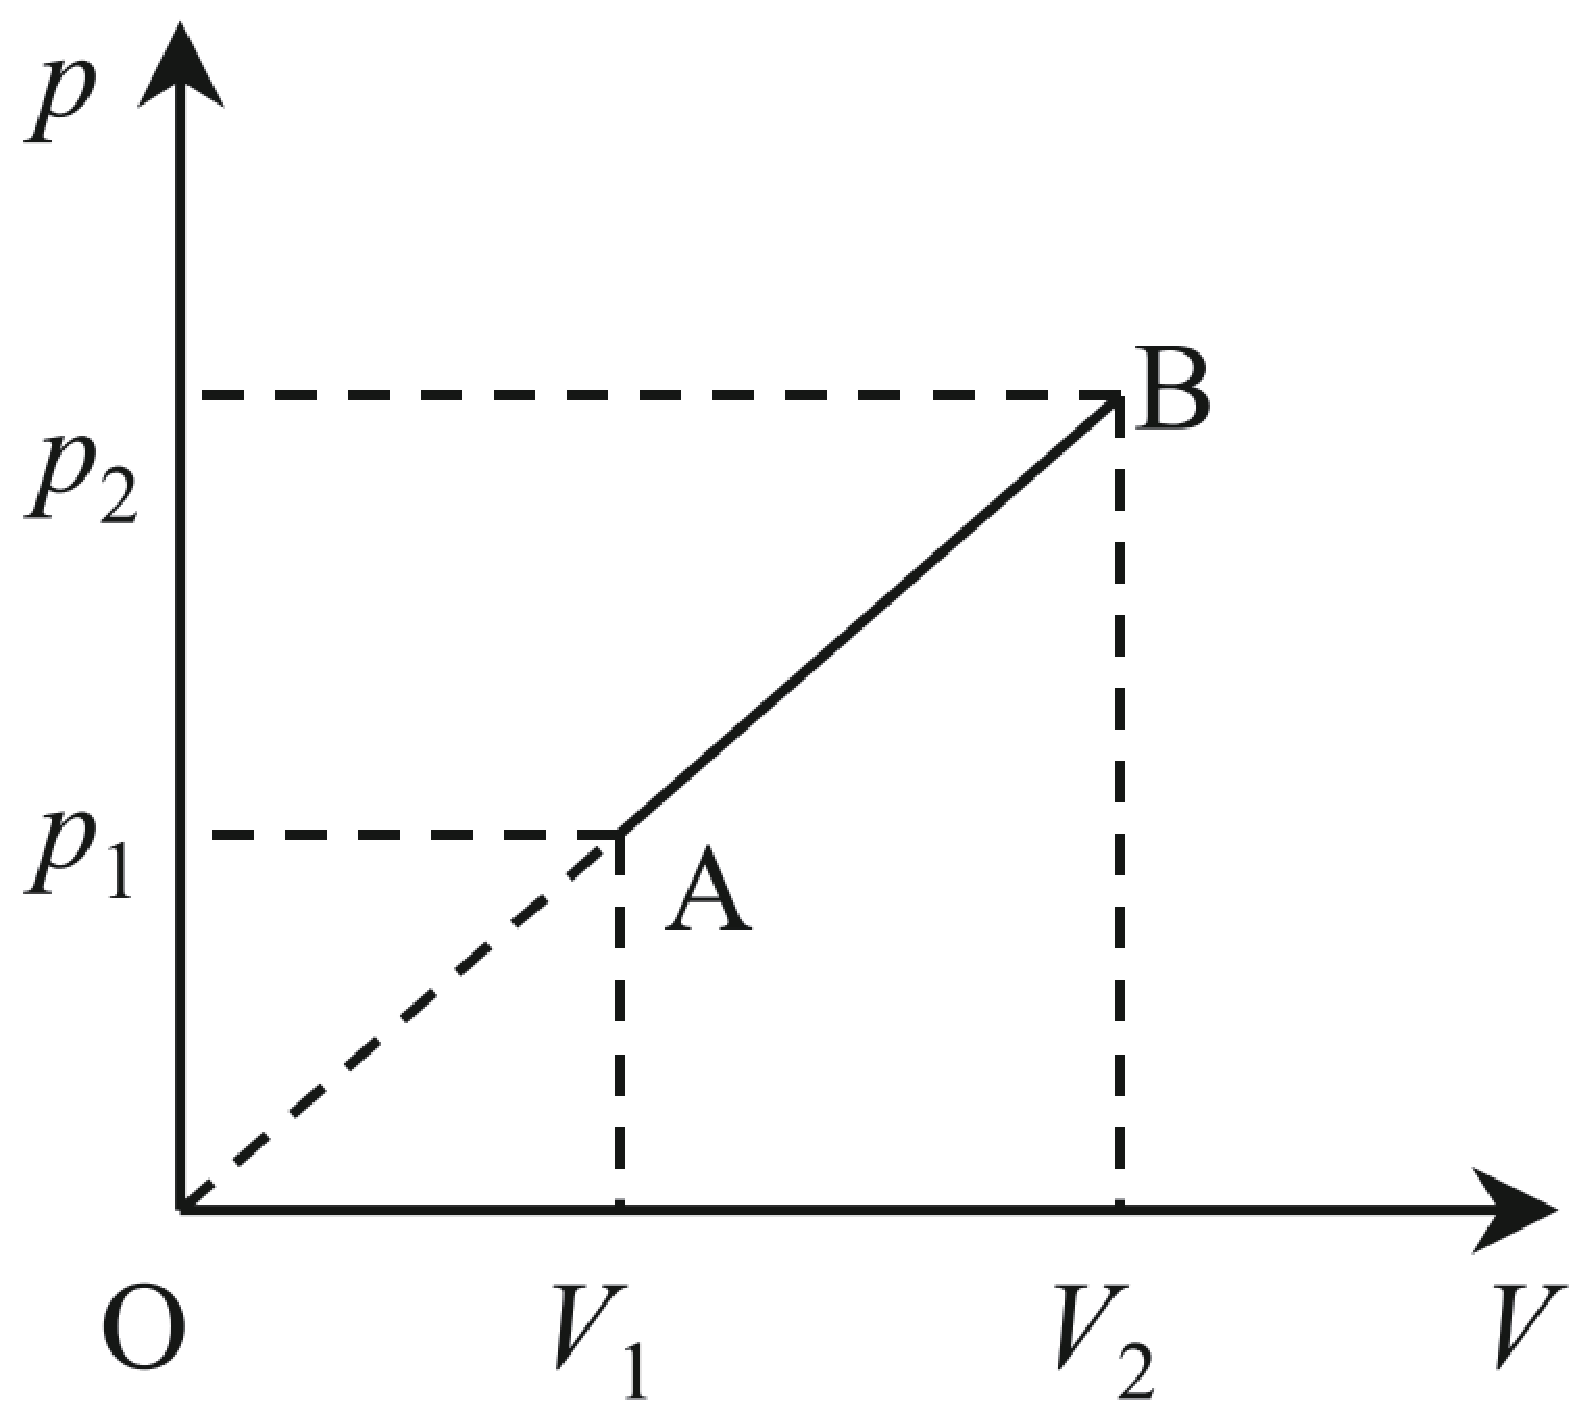
\includegraphics[width = 0.3\textwidth]{images/thermal-11.pdf} 
		\end{flushright}
	\tagged{student}{\vspace*{2cm}}
	\begin{taggedblock}{teacher}
		\noindent
		解析:$3kV_2^2-3kV_1^2$
	\end{taggedblock}
\end{example}
%%%%%%%%%%%%%%%%%%%%

%%%%%%%%%%%%%%%
\begin{example}
	如图,导热性能良好的气缸A和B高度均为$h$(已除开活塞的厚度),横截面积不同,竖直浸没在温度为$T_0$的恒温槽内。
	它们的底部由—细管连通(细管容积可忽略).两气缸内各有一个活塞,质量分别为$m_A=2m$和$m_B=m$,活塞与气缸之间无摩擦,两活塞的下方为理想气体,上方为真空。
	当两活塞下方气体处于平衡状态时,两活塞底面相对于气缸底的高度均为$h/2$。
	现保持恒温槽温度不变,在两活塞土上面同时各缓慢加上同样大小的压力,让压力从零缓慢增加,直至其大小等于$2mg$($g$为重力加速度)为止。
	并一直保持两活塞上的压力不变;系统再次达到平衡后,缓慢升高恒温槽的温度,对气体加热,直至气缸B中活塞底面恰好回到高度为$h/2$处.求
	
	1. 两个活塞的横截面积之比$S_A:S_B$,
	
	2. 气缸内气体的最后的温度;
	
	3. 在加热气体的过程中.气体对活塞所做的总功。
	
			\begin{flushright}
				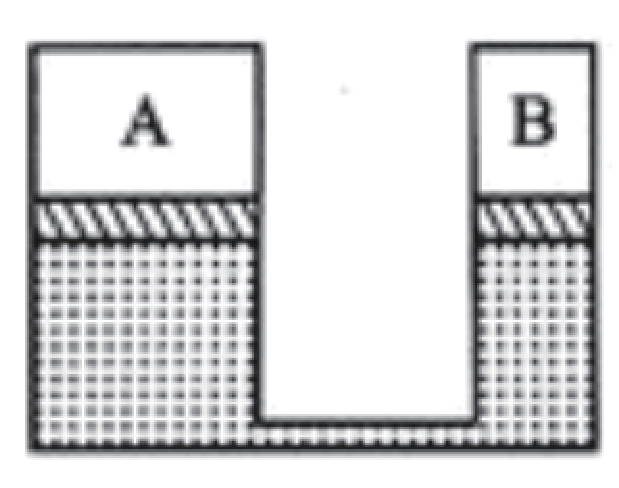
\includegraphics[width = 0.3\textwidth]{images/thermal-22.pdf} 
			\end{flushright}
	 
	\tagged{student}{\vspace*{2cm}}
	\begin{taggedblock}{teacher}
		\noindent
		解析:1.$S_A:S_B=2:1$
		\\2.$T=5T_0$
		\\3.$W=4mgh$
	\end{taggedblock}
\end{example}%%%
%%%%%%%%%%%%%%$$


\subsection{气体绝热过程}
如果气体状态变化过程当中与外界的热量交换为零或忽略不计,我们称该过程为{\heiti 绝热过程}(adiabatic process)。
根据热力学第一定律,绝热过程当中气体内能的减少量全部用来向外作功;反之外界对气体所作的功全部用来增加气体的内能。

下面的讨论仅限于准静态的绝热过程,在准静态的绝热过程中,作功可以按照$\Delta W = -p \Delta V$计算。

设给定数量的理想气体处于压强和体积分别为$p$和$V$的初始状态,在经过一个无穷小的绝热过程之后压强和体积分别变为$p+\Delta p$以及$V+\Delta V$,该绝热过程前后温度由$T$变成了$T+\Delta T$,根据热力学第一定律我们有
\begin{equation}
\Delta Q = \Delta U-\Delta W = \nu c_V\Delta T +p\Delta V = 0.
\end{equation}
在初态和末态气体都满足状态方程\ref{eqn: thermol 理想气体状态方程},可以得到各个状态参数变化量之间的一个关系
\begin{equation}
p\Delta V +V\Delta p = \nu R\Delta T.
\end{equation}
联立以上两式,消去所有和温度有关的量可以得到无限小绝热过程中压强和体积改变量$\Delta p$和$\Delta V$之间的一个关系:
\begin{equation}
\frac{\Delta p}{p}+\frac{c_V+R}{c_V}\frac{\Delta V}{V}=\frac{\Delta p}{p}+\frac{c_p}{c_V}\frac{\Delta V}{V}=0
\end{equation}
满足这一条件的 $p-V$关系称为绝热{\heiti 过程方程}(process function),可以证明理想气体的绝热方程为
\begin{equation}\label{eqn: thermol 绝热方程}
pV^\gamma = const,
\end{equation}
其中$\gamma = c_p/c_V$.





%%%%%%%%%%%%%%
\begin{example}
	利用理想气体状态方程证明对于理想气体,证明绝热过程方程\ref{eqn: thermol 绝热方程}还可以写成包含温度的形式
	\[TV^{\gamma-1} = const.\]
	\tagged{student}{\vspace*{2cm}}
	\begin{taggedblock}{teacher}
		\noindent
		解析:略
	\end{taggedblock}
\end{example}
%%%%%%%%%%%%%%%%%%%

%%%%%%%%%%%%%%%%%%
\begin{example}
如图所示,在一个质量为$M$、内部横截面积为$ A$的竖直放置的绝热气缸中,用活塞封闭了一定量温度度为$T_0$的理想气体。
活塞也是绝热的,活塞质量以及活塞和气缸之间的摩擦力都可忽略不计。
已知大气压强为$p_0$,重力加速度为$g$,现将活塞缓慢上提,当活塞到达气缸开口处时,气缸刚好离开地面。
求得活塞到达气缸开口处时气体的温度为多少?
	\begin{flushright}
		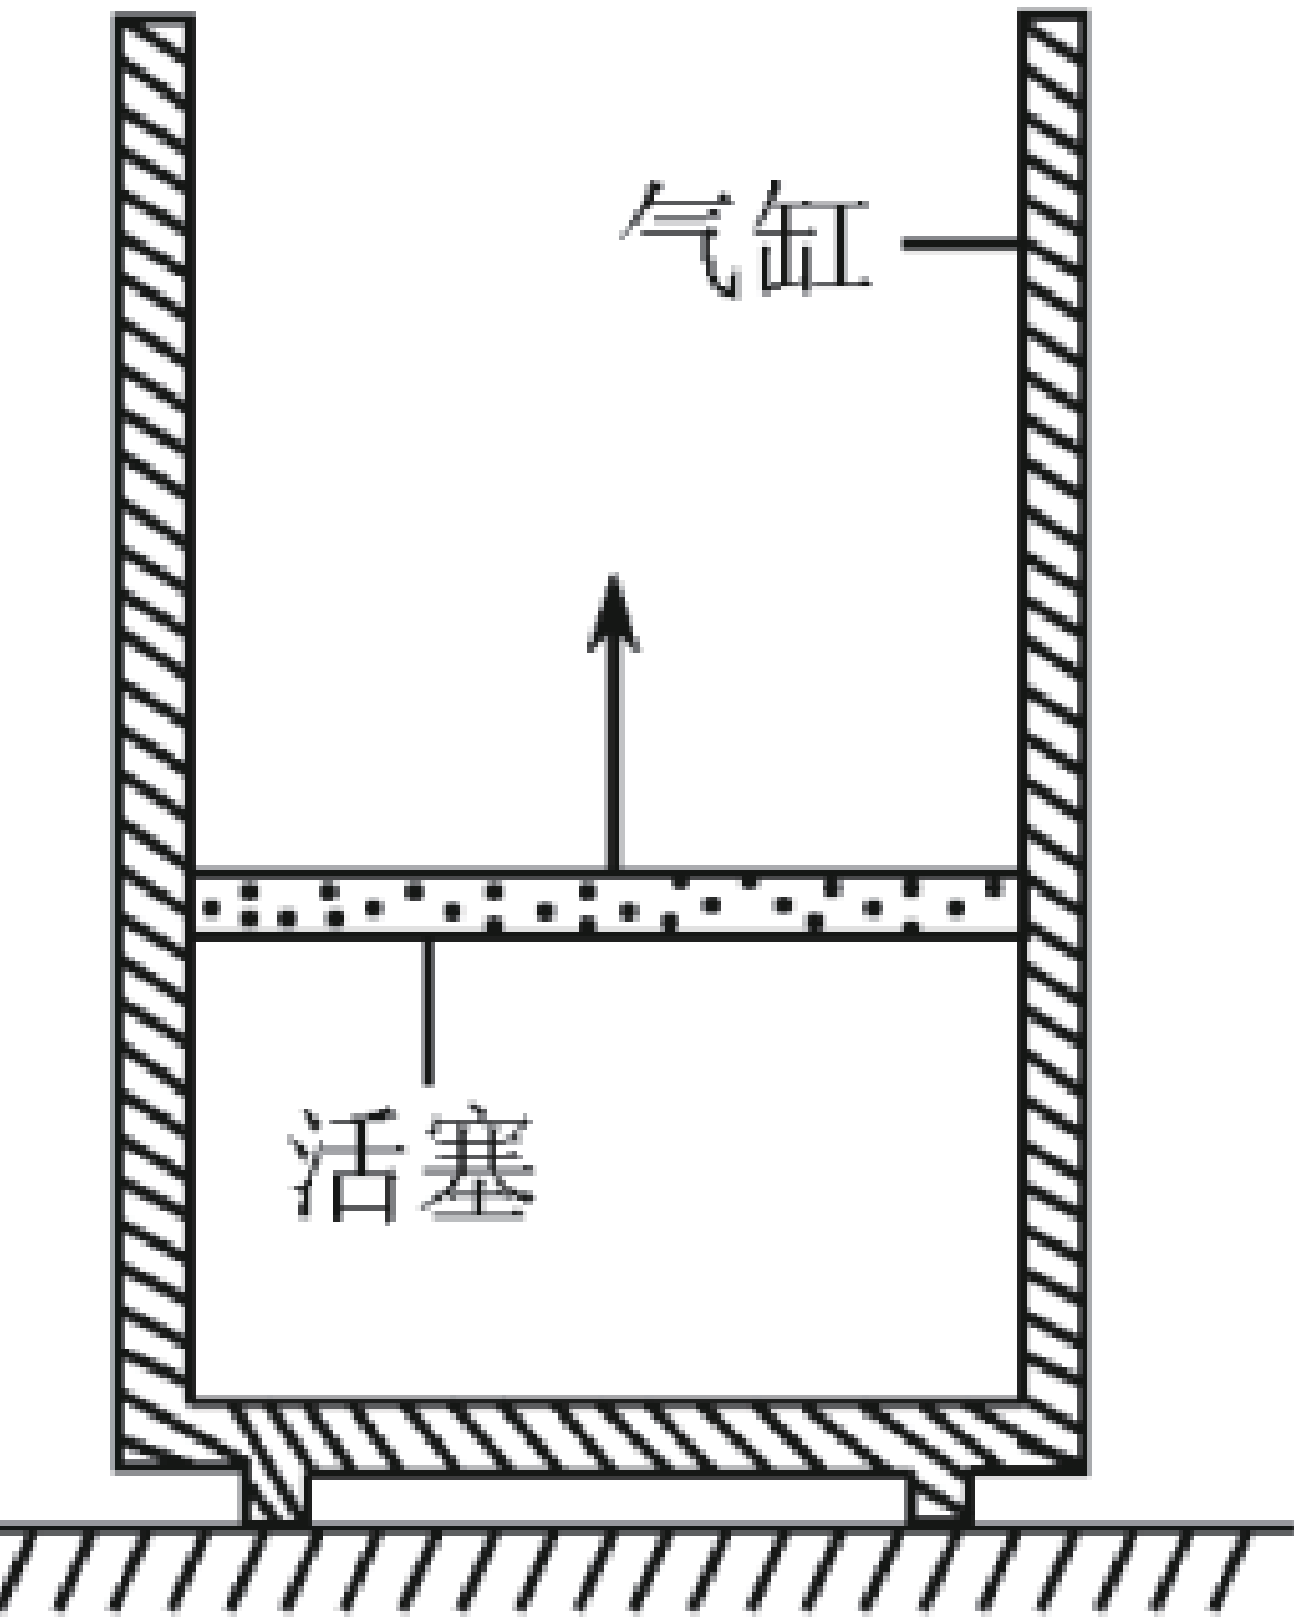
\includegraphics[width = 0.3\textwidth]{images/thermal-16.pdf} 
	\end{flushright}
\tagged{student}{\vspace*{0cm}}
\begin{taggedblock}{teacher}
\noindent
解析:$T_0(1-\frac{Mg}{p_0A}^\frac{\gamma-1}{\gamma})$
\end{taggedblock}
\end{example}
%%%%%%%%%%%%%%

%%%%%%%%%%%%%%%%
\begin{example}
理想气体经历如\ref{eqn: thermol 绝热方程}所给出的绝热过程,其中常数为已知量$C$,求由体积$V_1$绝热膨胀到$V_2$过程中对外所做的功。
\tagged{student}{\vspace*{4cm}}
\begin{taggedblock}{teacher}
\newline
解析:$W=-C_v*(T_1-T_2)=\frac{p_1V_1-p_2V_2}{\gamma-1}$
\end{taggedblock}
\end{example}
%%%%%%%%%%%%%%%%%%%%%

%%%%%%%%%%%%%
\begin{example}
	图中所示的气缸壁是绝热的.缸内隔板 A是导热的,它固定在缸壁上.活塞B 是
	绝热的,它与缸壁的接触是光滑的,但不漏气.B 的上方为大气.A与B 之间以及 A 与缸底之间都盛有$n\si{mol}$的同种理想气体.系统在开始时处于平衡状态.现通过电炉丝E 对气体缓慢加热.在加热过程中,A、B 之间的气体经
	历\kong 过程,A以下气体经\kong 过程;气体温度每上升1K, A、B 之间的气体吸收的热量与 A以下气体净吸收的热量之差等于\kong .已知普适气体常量为$R$ .
	\begin{flushright}
		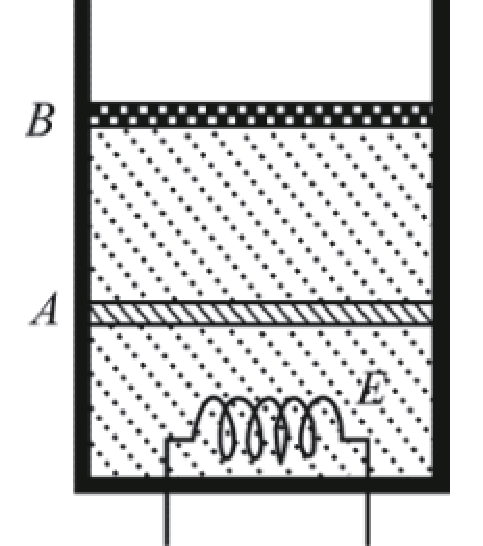
\includegraphics[width = 0.2\textwidth]{images/thermal-8.pdf} 
	\end{flushright}
	
	\begin{taggedblock}{teacher}
		\noindent
		解析:等压,  等容,  $nR$.
	\end{taggedblock}
\end{example}
%%%%%%%%%%%%%%%%%%%%

\subsection{热力学循环的效率}
当理想气体,或其它物质由某一特定状态出发经过一系列热力学过程之后又回到初始态,我们称它经历了一个热力学{\heiti 循环}(cyclic process, circle)。
以气体为例,气体作为{\heiti 工作物质}(working body)在一个循环的过程当中,它可能吸收了一定的热量,并向外作了一定数量的功,最终又放出了一些热量\footnote{在后面将会看到,不存在只吸热和作功的热力学循环}。这时这个体系称为{\heiti 热机}(heat engine)
这时气体对外作功与吸收热量的比值就是一个很有意义的物理量,称为热机的{\heiti 效率}(efficiency)。
对于一个给定的循环,它从外界吸收了$Q_1$的热量,对外做功$W$,最后又放出了$Q_2$的热量,根据热力学第一定律\ref{eqn: thermol 热力学第一定律}
\begin{equation}
Q_1=W+Q_2,
\end{equation}
很容易得到热机的效率为
\begin{equation}
\eta = \frac{W}{Q_1} = 1-\frac{Q_2}{Q_1}.
\end{equation}

\begin{example}
求$\nu \si{mol}$单原子理想气体经历如图所示的循环效率,其中所有未知量均已在图中标出。
	\begin{flushright}
		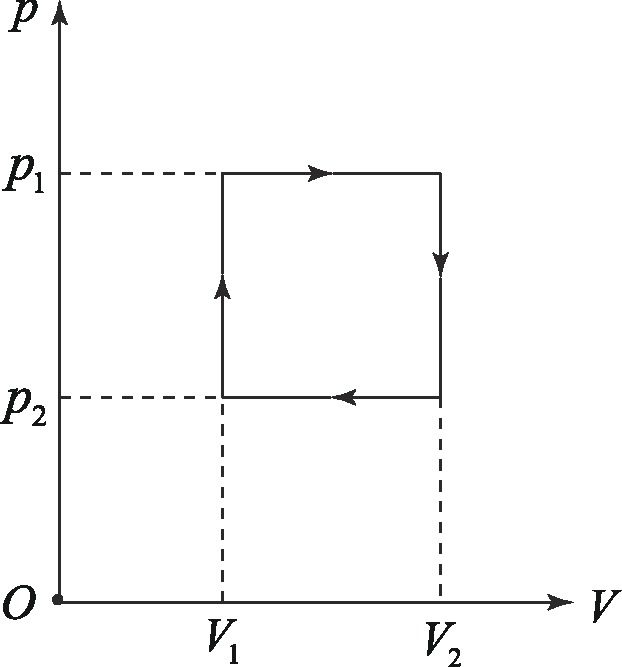
\includegraphics[width = 0.3\textwidth]{images/thermal-17.pdf} 
		\end{flushright}
\tagged{student}{\vspace*{2cm}}
\begin{taggedblock}{teacher}
\noindent
解析:$\eta=\frac{W}{Q}=\frac{2(p_1-p_2)*(v_2-v_1)}{5p_1(V_2-V_1)+3V_1(p_1-p_2)}$
\end{taggedblock}
\end{example}


\begin{example}
如图所示著名的卡诺循环,其中$1\rightarrow 2$,$3\rightarrow 4$为温度分别为$T_{1,2}$的等温过程,$2\rightarrow 3$,$4\rightarrow 1$则是连接两等温过程的绝热过程,试求卡诺循环的效率。
	\begin{flushright}
		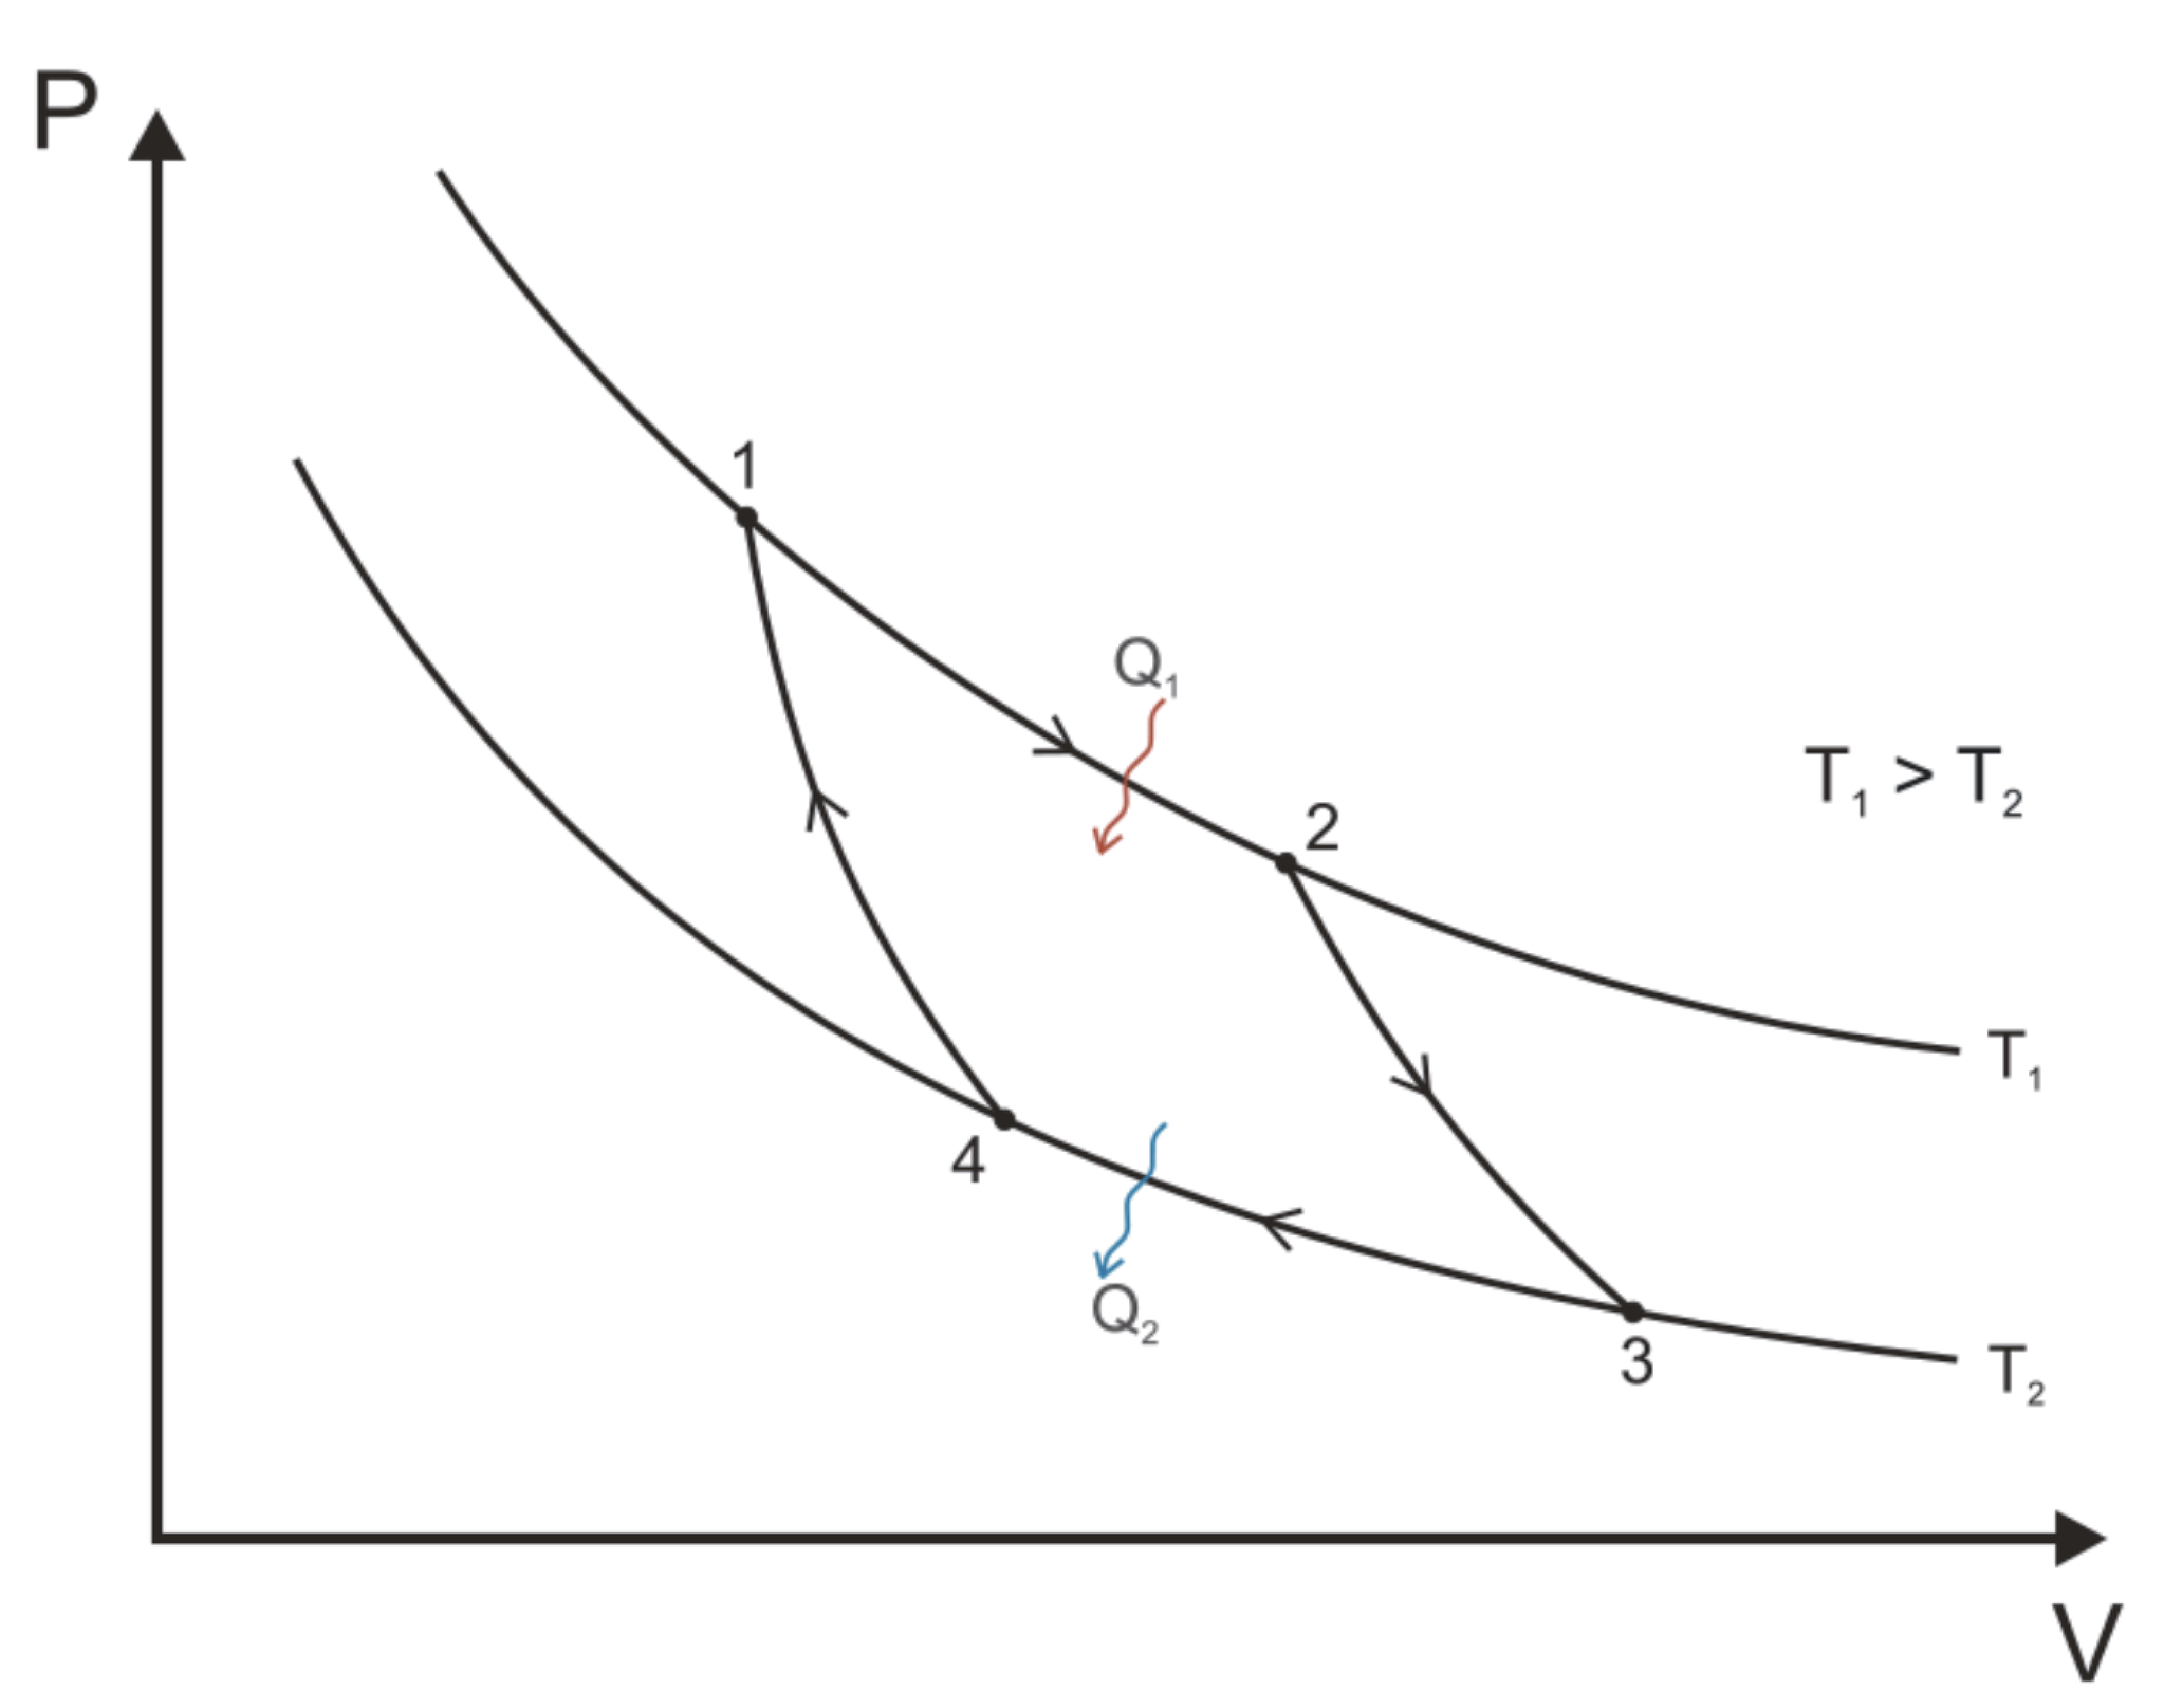
\includegraphics[width = 0.4\textwidth]{images/thermal-15.pdf} 
	\end{flushright}
\tagged{student}{\vspace*{2cm}}
\begin{taggedblock}{teacher}
\noindent
解析:$1-\frac{T_2}{T_1}$
\end{taggedblock}
\end{example}

\begin{example}
	一定量的理想气体经历如图所示的循环过程,$A\rightarrow B$ 和$C\rightarrow D$是等压过程$B\rightarrow C$和 $D\rightarrow A$是绝热 过程.已知:$T_C=$ 300 K,$T_B=$ 400 K. 试求:此循环的效率.
		\begin{flushright}
			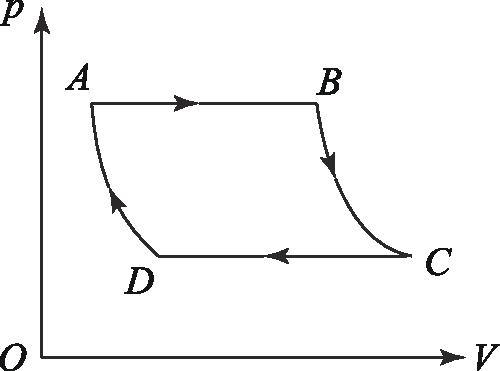
\includegraphics[width = 0.3\textwidth]{images/thermal-13.pdf} 
		\end{flushright}
	\tagged{student}{\vspace*{2cm}}
	\begin{taggedblock}{teacher}
	\noindent
		解析:$25\%$
	\end{taggedblock}
\end{example}

%%%%%%%%%%%%%
\begin{example}
	定容摩尔热容量$c_v$为常量的某理想气体,经历如图所示的$ p-V$平面上的两个循环过程$A_1B_1C_1A_1$和$A_2B_2C_2A_2$,相应的效率分别为$\eta_1$和$\eta_2$,试比较两循环效率。
	\begin{flushright}
		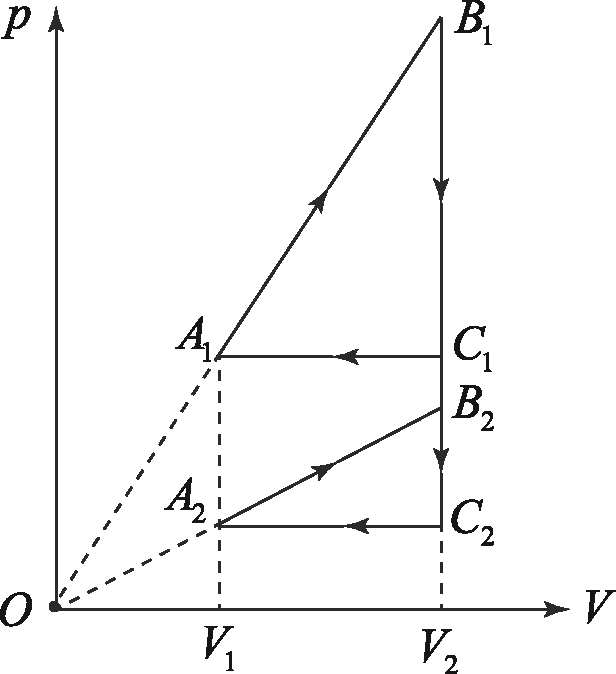
\includegraphics[width = 0.3\textwidth]{images/thermal-14.pdf} 
	\end{flushright}
	\tagged{student}{\vspace*{2cm}}
	\begin{taggedblock}{teacher}
		\noindent
		解析:一样
	\end{taggedblock}
\end{example}
%%%%%%%%%%%%%%%%%%%%


热机吸收热量对外作功,熟悉的蒸气机、内燃机就是典型的热机。
除此之外还有另一些与热机工作原理相似的机器,它们是通过外力对工作物质作功将热量从低温热源搬运到高温热源,如向{\heiti 热库}(heat sink)输送热量的\emph{热泵}(heat pump)与从低温热源抽取热量的\emph{制冷机}(refrigerator)。
衡量热泵和制冷机的效率有很多方式,其中最直观为{\heiti 性能系数}\footnote{也称制热系数,制冷系数}(coefficient of performance),它被定义为搬运的热量与外力作功的比值。

\begin{example}
卡诺循环的逆循环可以将热量由低温热源$T_2$传至高源热源$T_1$,可以看做一个理想的制冷机,根据定义计算它的制冷系数。
\tagged{student}{\vspace*{4cm}}
\begin{taggedblock}{teacher}
\newline
解析:$\frac{T_2}{T_2-T_1}$
\end{taggedblock}
\end{example}


\section{复杂气体过程}
在前面主要研究封闭在容器当中的气体,实际上真实发生的气体过程要远比它们复杂,有可能发生变化的物理量有时也会增加,下面我们就来看几种典型的稍复杂的气体过程。


很多情况下容器内气体的数量是会发生变化的,例如气体的混合或泄露、水气的蒸发和凝结、化学反应等等。
这时在使用理想气体状态方程\ref{eqn: thermol 理想气体状态方程}时就要注意不但气体的压强、体积和温度在热力学过程前后会发生变化,气体的摩尔数同样有可能发生变化。


%%%%%%%%%%%%%
\begin{example}
	由双原子分子构成的气体,当温度升高时,一部分双原子分子会分解成两个单原子分子,温度越高,被分解的双原子分子的比例越大,于是整个气体可视为由单原子分子构成的气体与由	双原子分子构成的气体的混合气体。
	这种混合气体的每一种成分气体都可视作理想气体.在体积$	V=0.045m^3$的坚固的容器中,盛有一定质量的碘蒸气,现于不同温度下测得容器中蒸气的压强如下:$T=1073K$时$p = \num{2.099e5}\si{Pa}$,$T=1473K$时$p = \num{4.120e5}\si{Pa}$.
	试求温度分别为$ 1073K $和$ 1473K $时该碘蒸气中单原子分子碘蒸气的质量与碘的总质量之比值.已知碘蒸气的总质量与一个摩尔的双原子碘分子的质量相同.
	\tagged{student}{\vspace*{4cm}}
	\begin{taggedblock}{teacher}
		\noindent
		解析:$T=1073K,\alpha=0.06.  T=1473K,\alpha=0.51$
	\end{taggedblock}
\end{example}
%%%%%%%%%%%%%%%%%%%%




和封闭在容器内的气体不同的是,大部分气体实际上是存在于一个开放的环境当中,例如等离子体气体构成的太阳,随高度上升温度递减的对流层大气等等。
即使这些处于开放环境当中的气体可以当成理想气体来处理,也不能够直接使用理想气体的状态方程\ref{eqn: thermol 理想气体状态方程},因为此时无法定义气体的体积。
如果只有同种气体时我们将状态方程当中的体积$V$搬到方程的右边,并同时乘以和除以该种气体的摩尔质量$\mu$,这样状态方程变成了
\begin{equation}
p = \frac{\nu \mu}{V}\frac{R}{\mu}T = \frac{m}{V}\frac{R}{\mu}T,
\end{equation}
简单的观察可以发现上式右边第一个分式不是别的,正是气体的密度$\rho$,这时状态方程被解释为气体的压强$p$、密度$\rho$以及温度$T$之间的一个关系:
\begin{equation}
p=\frac{\rho}{\mu}R T.
\end{equation}
利用上式则可以研究开放系统中的气体。
如果需要处理的是混合气体,此时{\heiti 道尔顿分压定律}(\textit{Dalton\,}'s Law of Partial Pressures)依然成立,状态方程则相应地变为
\begin{equation}
p = \left(\sum_{i=1}^N \frac{\rho_i}{\mu_i}\right)RT,
\end{equation}
其中$\rho_i$和$\mu_i$分别为第$i$种组分的密度以及摩尔质量。

这种情况下,气体温度发生变化时内能也会做相应的变化,但此时定义单位体积内气体的内能更有实际意义。
对于单原子理想气体的内能
\begin{equation}
U = \frac{3}{2}\nu RT = \frac{3}{2}pV = \frac{3}{2}\frac{\rho}{\mu}RT V,
\end{equation}
这样单位体积的内能
\begin{equation}
u = \frac{U}{V} = \frac{3}{2}\frac{\rho}{\mu}RT,
\end{equation}
从中能够得到内能密度(单位体积的内能)与密度和温度的关系。
当气体膨胀时同样会向外作功,但是体积的变化实际上体现为气体密度的变化。
在密度和温度变化的过程中,热力学第一定律依然成立,因为它实际上就是能量的守恒定律。



%%%%%%%%%%%%%%%%
\begin{example}
密度为$\rho_1$、温度为$T_1$的摩尔质量为$\mu$的单原子理想气体缓慢绝热膨胀至密度为$\rho_2$的状态,试求此时气体的温度。
\tagged{student}{\vspace*{3cm}}
\begin{taggedblock}{teacher}
\newline
解析:绝热公式的简单应用,绝热过程中温度和压强的关系为
\[
\frac{T^\gamma}{p^{\gamma-1}}=const,
\]
利用用密度表示的理想气体状态方程$p \propto\rho T$ 代入上式可得
\[ \frac{T}{\rho^{\gamma-1}}=const\]
单原子气体$\gamma=5/3$,这样可以轻易解得
\[ T_2 = \left ( \frac{\rho_2}{\rho_1} \right )^{2/3}T_1 \]
\end{taggedblock}
\end{example}
%%%%%%%%%%%%%%%%%%



处于开放环境的气体有可能发生流动,由于气体的密度并不大,所以大多时候气体分子运动的动能可以忽略不计。
但对于有些问题来说气体的速度非常重要,例如飞机或火箭的发动机本身就是利用喷出的高速气体来工作的,这时气体的速度是绝不能够忽略不计的。
在这一类包含有高速运动气体的问题当中使用热力学第一定律时要特别注意的是气体的能量变化除了由于温度变化所造成的内能变化以外还应当包括由于气体的速度所导致的动能。



%%%%%%%%%%%%%%%%%%%%
\begin{example}
火箭通过高速喷射燃气产生推力。设温度$T_1$、压强$ p_1$的炽热高压气体在燃烧室内源源不断生成,并通过管道由狭窄的喷气口排入气压$ p_2$的环境。
假设燃气可视为理想气体,其摩尔质量为$\mu$,每摩尔燃气 的内能为$ u=c_vT$(c$c_v$常量,$T$为燃气的绝对温度)。
在快速流动过程中,对管道内任意处的两个非常靠近的横截面间的气体,可以认为它与周围没有热交换,但其内部则达到平衡状态,且有均匀的压强$ p$、温度
$T$和密度$\rho$,它们的数值随着流动而不断变化,并满足绝热方程
\[pV^{\frac{c_v+R}{c_v}}=C\]
其中$C$为常量,求喷气口处气体的温度与相对火箭的喷射速率。
\tagged{student}{\vspace*{4cm}}
\begin{taggedblock}{teacher}
\newline
解析:$v=\sqrt{\frac{2(c_v+R)T_1}{\mu}[1-(\frac{p_2}{p_1})^\frac{R}{C_v+R}]}$
\end{taggedblock}
\end{example}
%%%%%%%%%%%%%%%%%%%%%%

%%%%%%%%%%%%%%%%%%%
\begin{example}
炉内燃烧产生的气体通过高度为$h$截面积为$S$的烟筒排入密度为$\rho_0$温度为$T_0$的空气当中。
固体燃料燃烧在单位时间里产生的气体体积为$B$、温度为$T_1$。
假设炉内燃烧产生气体的速度能够忽略不计,而且这些气体能够看做理想气体并且满足和空气相同的状态方程(相同的密度和温度时压强相同);烟筒内气体密度变化忽略不计,求燃烧产生气体能够完全排出所需要的烟筒的最低高度。
\tagged{student}{\vspace*{4cm}}
\begin{taggedblock}{teacher}
\newline
解析:物理的分析告诉我们,当气体能够顺利排出时炉内的压强应当就是大气压强,而在烟筒出口处的压强也是该处大气的压强,由于有一定的高度差所以与炉内的压强稍有不同。
烟筒需要一定的高度才能够使作用在内部气体上的压力足够大,这样气体才能获得更快的速度,在大气压力作用下向上运动,设当高度为$h$时烟在烟筒出口处的速度为$v$。
根据伯努力原理我们有
\[
p_0=(p_0-\rho_0 gh)+\rho_s g h +\frac{1}{2}\rho_s v^2
\]
这样很容易解出速度与其它物理量的关系:
\[
v=\sqrt{2gh\left(\frac{\rho_0}{\rho_s}-1\right)}
\]
其中$\rho_s$为气体在出口处的密度。
由于大气压强在烟筒的底部和顶部的差别其实非常之小,在此我们忽略它们的区别。
根据烟筒内部气体和空气的状态方程
\[
p_s = \frac{\rho_s}{\mu}RT_1,\qquad p_0 = \frac{\rho_0}{\mu}RT_0
\]
比较两式可得
\[  \frac{\rho_s}{\rho_0}=\frac{T_0}{T_1}  \]
代入速度的表达式
\[
v=\sqrt{2gh\left(\frac{T_1}{T_0}-1\right)}
\]
要想让所有的气体全部排出去我们要求$Sv\ge B$,该不等式的解为
\[ h\ge \frac{B}{2gS}\frac{T_0}{T_1-T_0} \]
上式右边除了烟筒的截面积以外都只与燃烧的性质有关,所以更有意义的结果为
\[ S h\ge \frac{B}{2g}\frac{T_0}{T_1-T_0} \]
可见产生气体越多,所需要的烟筒就越高或越粗!
\end{taggedblock}
\end{example}
%%%%%%%%%%%%%%%%%%%%%%%%%%%%%%





\section{热力学第二定律简介}
之前我们学过热机的效率,从中可以看到任何热机在吸热作功之后一般会将一定的热量释放出去,从而使得热机的效率都小于一。
那么能否通过精巧的设计来避免这一现象,做出一台只从一个热源吸热并且全部转化为机械功的热机呢?
这种类型的热机称做{\heiti 第二类永动机}(perpetual motion of the second kind),它并不违反热力学第一定律,在历史上很长一段时间里人们都致力于寻找和设计这样一种热机,但以失败而告终。
第二类永动机的失败暗示着新的热力学规律的存在,今天称其为{\heiti 热力学第二定律}(second law of thermodynamics)。

热力学第二定律的数学形式需要定义一个新的物理量--{\heiti 熵}(entropy)。
和内能一样,熵是热力学系统状态的函数,如果在状态发生变化过程中该热系统吸收或放出热量,那么它的熵会随之变化。 
对于一个处于温度为$T$的平衡态的热力学系统,在一个准静态过程中向其输入$\Delta Q$的热量之后,它的熵$S$会增加
\begin{equation}\label{eqn: thermol 熵增的定义}
\Delta S = \frac{\Delta Q}{T},
\end{equation}
反之放出热量它的熵的减小量也由上式给出,那时$\Delta Q<0$。
热力学第二定律告诉我们,一个\CJKunderwave{孤立系统}的熵不会减小:
\begin{equation}
\Delta S \ge 0,
\end{equation}
这就是所谓的{\heiti 熵增原理}。

可以证明热力学中的熵与构成物质系统原子分子的运动“混乱”程度有关,越混乱的系统熵越大,反之越有序的系统的熵则越小。
熵增原理就是说与外界隔绝的系统的内部运动是向着更加“混乱”的方向进行的。


\begin{example}
从熵增原理出发证明下列热力学第二定律其它表述方式的等价性:
\begin{description}
\item[开尔文表述]不可能制成一种循环动作的热机,从单一热源取热,使之完全变为功而不引起其它变化。
\item[克劳修斯表述]不可能把热量从低温物体传向高温物体而不引起其它变化。
\end{description}
\tagged{student}{\vspace*{3cm}}
\begin{taggedblock}{teacher}
\noindent
解析:1. 仅从单一热源吸热完全变成机械功,设吸热$\Delta Q$,热源的温度为$T$,这样熵的变化 $\Delta S = -\frac{\Delta Q}{T}<0$,违背熵增原理。

2. 设两个物体的温度分别为$T_{1,2}$,其中$T_1>T_2$。
有热量$\Delta Q$从低温传向高温,如果没有其它变化,这时熵的增加量
\[\Delta S =\frac{\Delta Q}{T_1}-\frac{\Delta Q}{T_2}=\Delta Q \left( \frac{1}{T_1}-\frac{1}{T_2} \right)<0\]
违背熵增原理,所以不可能。
\end{taggedblock}
\end{example}

\begin{example}
试通过热力学第二定律说明,在高温热源$T_1$和低温热源$T_2$之间工作的各种热机的效率不会高于卡诺热机。
\tagged{student}{\vspace*{4cm}}
\begin{taggedblock}{teacher}
\newline
解析:设从高温热源吸热$Q_1$,向低温热源放热$Q_2$,由热力学第二定律
\[  \Delta S = -\frac{Q_1}{T_1}+\frac{Q_2}{T_2}\ge 0  \]
可得
\[  Q_2 \ge Q_1 \frac{T_2}{T_1}, \]
根据热机效率的定义
\[  \eta = 1-\frac{Q_2}{Q_1}\le 1-\frac{T_2}{T_1}\]
\end{taggedblock}
\end{example}

虽然无法直接确定绝对的熵,但通过熵的定义\ref{eqn: thermol 熵增的定义}出发可以求出两个状态之间熵的差别:
\begin{example}
对于$\nu$摩尔理想气体,已知其摩尔等容热容量为常数$c_V$。
如果它在体积为$V_0$,温度为$T_0$的状态的熵为$S_0$,求它在体积为$V$,温度为$T$时的熵。
并由此出发说明为什么处于封闭容器内的气体分子不会自发地聚集在容器的一侧。
\tagged{student}{\vspace*{4cm}}
\begin{taggedblock}{teacher}
\newline
解析:气体的状态发生变化时,根据热力学第二定律,吸收的热量为
\[ 
\Delta Q = \nu c_V\Delta T+p\Delta V,
\]
从理想气体的状态方程当中解出压强
\[
p = \frac{\nu RT}{V}
\]
根据熵的定义\ref{eqn: thermol 熵增的定义},并将压强代入可得
\[
\Delta S = \nu c_V\frac{\Delta T}{T}+\nu R\frac{\Delta V}{V},
\]
将它积分
\[
S(V,T)-S(V_0,T_0)=S(V,T)-S_0 = \nu c_V\ln\frac{T}{T_0}+\nu R\ln\frac{V}{V_0}
\]
对于相同温度不同体积的理想气体,体积越大熵越大,根据熵增原理,气体不会自发地聚集于容器的一侧。
\end{taggedblock}
\end{example}









\section{液体表面张力、毛细现象}
处于液体表面的分子与内部的分子有所不同,它们将受到不平衡的分子力,体现为一个向内的吸引力。
这样宏观上看液体的表面就有收缩的趋势,体现为液体的{\heiti 表面张力}(surface tension)。
表面张力现象从处于太空当中失重的水珠很容易看到,太空当中的水珠均处于球形,因为所有体积相同的物体球形的表面为最小。

细致地分析液体表面扩张过程可以发现其实是有一定的能量储存于液体表面,将这种能量称为液体的{\heiti 表面能}(surface energy)。
很容易证明液体表面能的大小与液体本身的性质(分子作用力)有关,且正比于液体的表面积:
\begin{equation}\label{eqn: thermol 表面能}
E_S = \sigma S
\end{equation}
其中$S$为液体表面积,$\sigma$称作表面张力系数。
由于表面能的存在,当试图扩大液体表面积时需要外力作功。
对于缓慢的表面积扩大过程,外力所做的功完全用来提供表面能,根据这个性质可以确定表面张力的大小和方向。
例如在两根相距$l$的平行铁丝中间有一个肥皂泡,在外力$F$作用下边界向右移动了$\Delta x$的距离,在这个过程中外力作功$W=F\Delta x$,与此同时液体表面扩大了$2l\Delta x$,这其中的因子2是因为肥皂膜有上下两个表面。
根据表面能的表达式\ref{eqn: thermol 表面能},表面能量有所增加,由能量守恒我们有
\begin{equation}
F\Delta x = 2\sigma l\Delta x,\qquad F = 2\sigma l
\end{equation}
可得表面张力的大小,在这个例子中张力的方向容易判定,对于更一般的情况来说,表面张力的方向平行于液面,指向使液体表面收缩的方向。


\begin{example}
绷紧的肥皂薄膜有两个平行的边界,线 AB 将薄膜分隔成两部分。
为了演示液体的表面张力现象,刺破左边的膜,线 AB 受到表面张力作用被拉紧,试求此时线的张力。
两平行边之间的距离为$d$,线 AB 的长度为 $l$($l> \pi d/2$),肥皂液的表面张力系数$\sigma$。
\begin{flushright}
\includegraphics[width=0.3\textwidth]{images/mebrane-1.pdf}
\end{flushright}

\tagged{student}{\vspace*{1cm}}
\begin{taggedblock}{teacher}
\noindent
解析:液体表面能正比于其表面积,自然状态下所有物理系统都会最终变成能量最小的状态。
所以最终的平衡状态是液体表面积在所有可能情况下为最小的状态。
对于这个问题,可能的面积最小状态如图所示,绳子先是平行于边界,然后形成一个半圆形。


\includegraphics[width=0.9\textwidth]{images/mebrane-2.pdf}

绳子上的张力可以用力或能量的方法求出。
如果用力的方法会比较麻烦。对于如图所示的一小段,张力的方向沿着半圆半径方向向外,它们与绳子里的张力平衡。
由于张力处处相等,所以我们有
\[
T\Delta \theta = 2\sigma r \Delta \theta
\]
这样可得$T = 2\sigma r = \sigma d.$

如果用能量的方法,可以利用虚功原理:设想沿着绳子的方向将液体膜拉开$\Delta x$的距离,根据作功等于表面能的增量可得
\[ 2T\Delta x = 2\sigma d\]
同样可以得到和用力学方法相同的结论。
\end{taggedblock}
\end{example}

\begin{example}
有一个放置于真空当中半径$r=5\unit{cm}$的肥皂泡内部包含有某种双原子理想气体,泡的厚度$h=10\unit{\mu m}$,泡泡的表面张力系数$\sigma=4\pow{-2}\unit{N/m}$,密度$\rho = 1.10 \unit{g/m^3}$。
求该肥皂泡的摩尔热容量,假设泡泡加热极其缓慢使得其时刻处于力学平衡状态。
\tagged{student}{\vspace*{4cm}}
\begin{taggedblock}{teacher}
\newline
解析:$p=\frac{4\sigma}{r}$,    $\frac{5R}{2}+\frac{P*dV}{dT}=\frac{5R}{2}+\frac{3R}{2}=4R$
\end{taggedblock}
\end{example}

\begin{example}
如图所示竖直放置的滴定管,内直径为$d$。
水缓慢地由上部注入,设水的密度为$\rho$,其表面张力系数为$\sigma$。
当水滴的半径超过$r_{max}$时它将会掉落下来,假设$d\ll r_{max}$,求水滴落下时的半径。
\begin{flushright}
\includegraphics[width=0.3\textwidth]{images/water-drop.pdf}
\end{flushright}
\tagged{student}{\vspace*{2cm}}
\begin{taggedblock}{teacher}
%\newline
\begin{center}
\includegraphics[width=0.3\textwidth]{images/water-drop-1.pdf}
\end{center}
\noindent
解析:这是IPhO当中的一个问题,如图所示假设在外力$F$作用下使得水珠下降$\Delta x$的距离,$\Delta x$极其之小,忽略重力势能的变化,这样液体的表面积扩大了$\pi d\Delta x$。
根据表面张力能量的决定式\ref{eqn: thermol 表面能}表面能量增加了$\sigma \pi d\Delta x$。
外力作功等于该能量的增加值
\[
F\Delta x = \sigma \pi d\Delta x
\]
可以解出此时表面张力的大小$F=\sigma \pi d$。

能够看出液体表面张力贡献与液滴的大小无关,当液滴增大时其重力增加,当半径增加到一定程度时表面张力不足以抵抗重力从而掉了下来。
这样液滴最大的半径$r_{max}$将满足
\[
\sigma \pi d = \rho g\frac{4}{3} \pi r_{max}^3,\qquad r_{max} = \left(\frac{3\sigma d}{4\rho g}\right)^{1/3} .
\]
\end{taggedblock}
\end{example}

\begin{example}
如图,一个上端固定、内半径为$R_1$的玻璃圆筒底部浸没在大容器中的水面之下,未与容器底接触;另将一个外半径为$R_2$(略小于$R_1$)的同质玻璃圆筒(上端固定)放置其中,不接触容器底,保持两玻璃圆筒的中轴线重合且竖直。
设水与玻璃之间的接触角为$\theta$(即气、液界面在水的最高处的切线与固、液界面的夹角,见局部放大图)。
已知水的表面张力系数为$\sigma$,地面重力加速度大小为$g$。

在毛细现象中,系统毛细作用引起的势能变化,可以等效地看作固、液、气分界线上液体表面张力在液面上升或下降过程中做的功。
并求出平衡时液体的高度$h$.
\begin{flushright}
\includegraphics[width=0.3\textwidth]{images/height-problem.pdf}
\end{flushright}
\tagged{student}{\vspace*{3cm}}
\begin{taggedblock}{teacher}
\noindent
解析:本题为2015年决赛题,由几何关系表面张力能够提供向上的拉力为
\[
F = 2\pi \sigma (R_1+R_2)\cos\theta
\]
而高度为$h$的液体的总重力则是
\[
\rho g \pi(R_1^2-R_2^2)h
\]
容易得到平衡时液体的高度为
\[
h=\frac{2\sigma \cos\theta}{\rho g (R_1-R_2)}
\]
可见两者半径相关越小液体则升得越高,这和通常的毛细现象定性的结论也是一样的。
\end{taggedblock}
\end{example}

\section{固体知识简介}




\section{相变}
理想气体模型当中包含着一条非常重要的假设,即气体分子之间没有相互作用力。
事实上分子之间不但有相互作用力,而且正是由于分子间作用力的存在才使得我们拥有一个丰富多彩的物质世界。
当分子之间距离较远时它们之间表现为范德瓦尔斯(J.D. van de Waals)吸引力,反之在外力压缩下当分子彼此靠近试图进一步缩小之间距离时则会表现为泡利(Wolfgang E. Pauli)排斥力。
由大量分子构成的物质形态是由分子间的作用力和分子的热运动共同决定的。
相互作用倾向于使分子成为有序的状态,相反热运动则会使物质处于相对无序的状态,最终物质所处的状态,我们称之为{\heiti 相}(phase),是相互作用力与热运动对抗的结果。

在热运动的能量较小时,大量的分子(原子)就会处于由它们之间相互作用力所决定的平衡位置,分子只能在其平衡位置附近做由热运动所带来的小幅度振荡而不会运动到更远的地方,这时物质处于{\heiti 固态}(solid state)。
当物质吸收热量温度升高时,分子热运动将越来越大,当温度达到一定程度是有可能分子的平均动能超过平衡位置处的势阱,这时分子就有可能四处运动,但彼此之间的距离和固态相当,这样的状态就是熟悉的{\heiti 液态}(liquid state)。
由于物质吸收热量而导致的固态向液态转变的过程被称为{\heiti 熔化}(melting),反过来液态物质当放出热量时会转变为固态,这一过程是熔化的逆过程,称为{\heiti 凝固}\footnote{在{\heiti 溶液}(solution)中,{\heiti 溶质}(solute)分散到{\heiti 溶质}(solvent)中的过程称为{\heiti 溶解}(dissolution),而溶质从溶液中聚集的过程则称为{\heiti 沉积}(precipitation)}(freezing)。

处于液态的物质如果进一步吸收热量,当温度达到一定程度以后分子的热运动的平均能量将超过每一对分子间作用力产生的势阱,这时任意两个分子都可以彼此完全分离而形成自由运动状态,这就是我们熟悉的{\heiti 气态}(gas state),通常情况下气态物质的密度远小于液态,这个过程被称为液体的{\heiti 汽化}(vaporization),汽化的逆过程则被称为气体的{\heiti 液化}(condensation)。
气体和液体只有在特定的温度和压强下才能够共存,可以在$p-T$图中将气液能够共存点连接起来,这样一条曲线称为{\heiti 汽化曲线}。

同理,物质吸收热量而导致的固态向气态转变的过程被称为{\heiti 升华}(sublimation);升华的逆过程为{\heiti 凝华}(deposition)。

\begin{figure}[h]
	\centering
	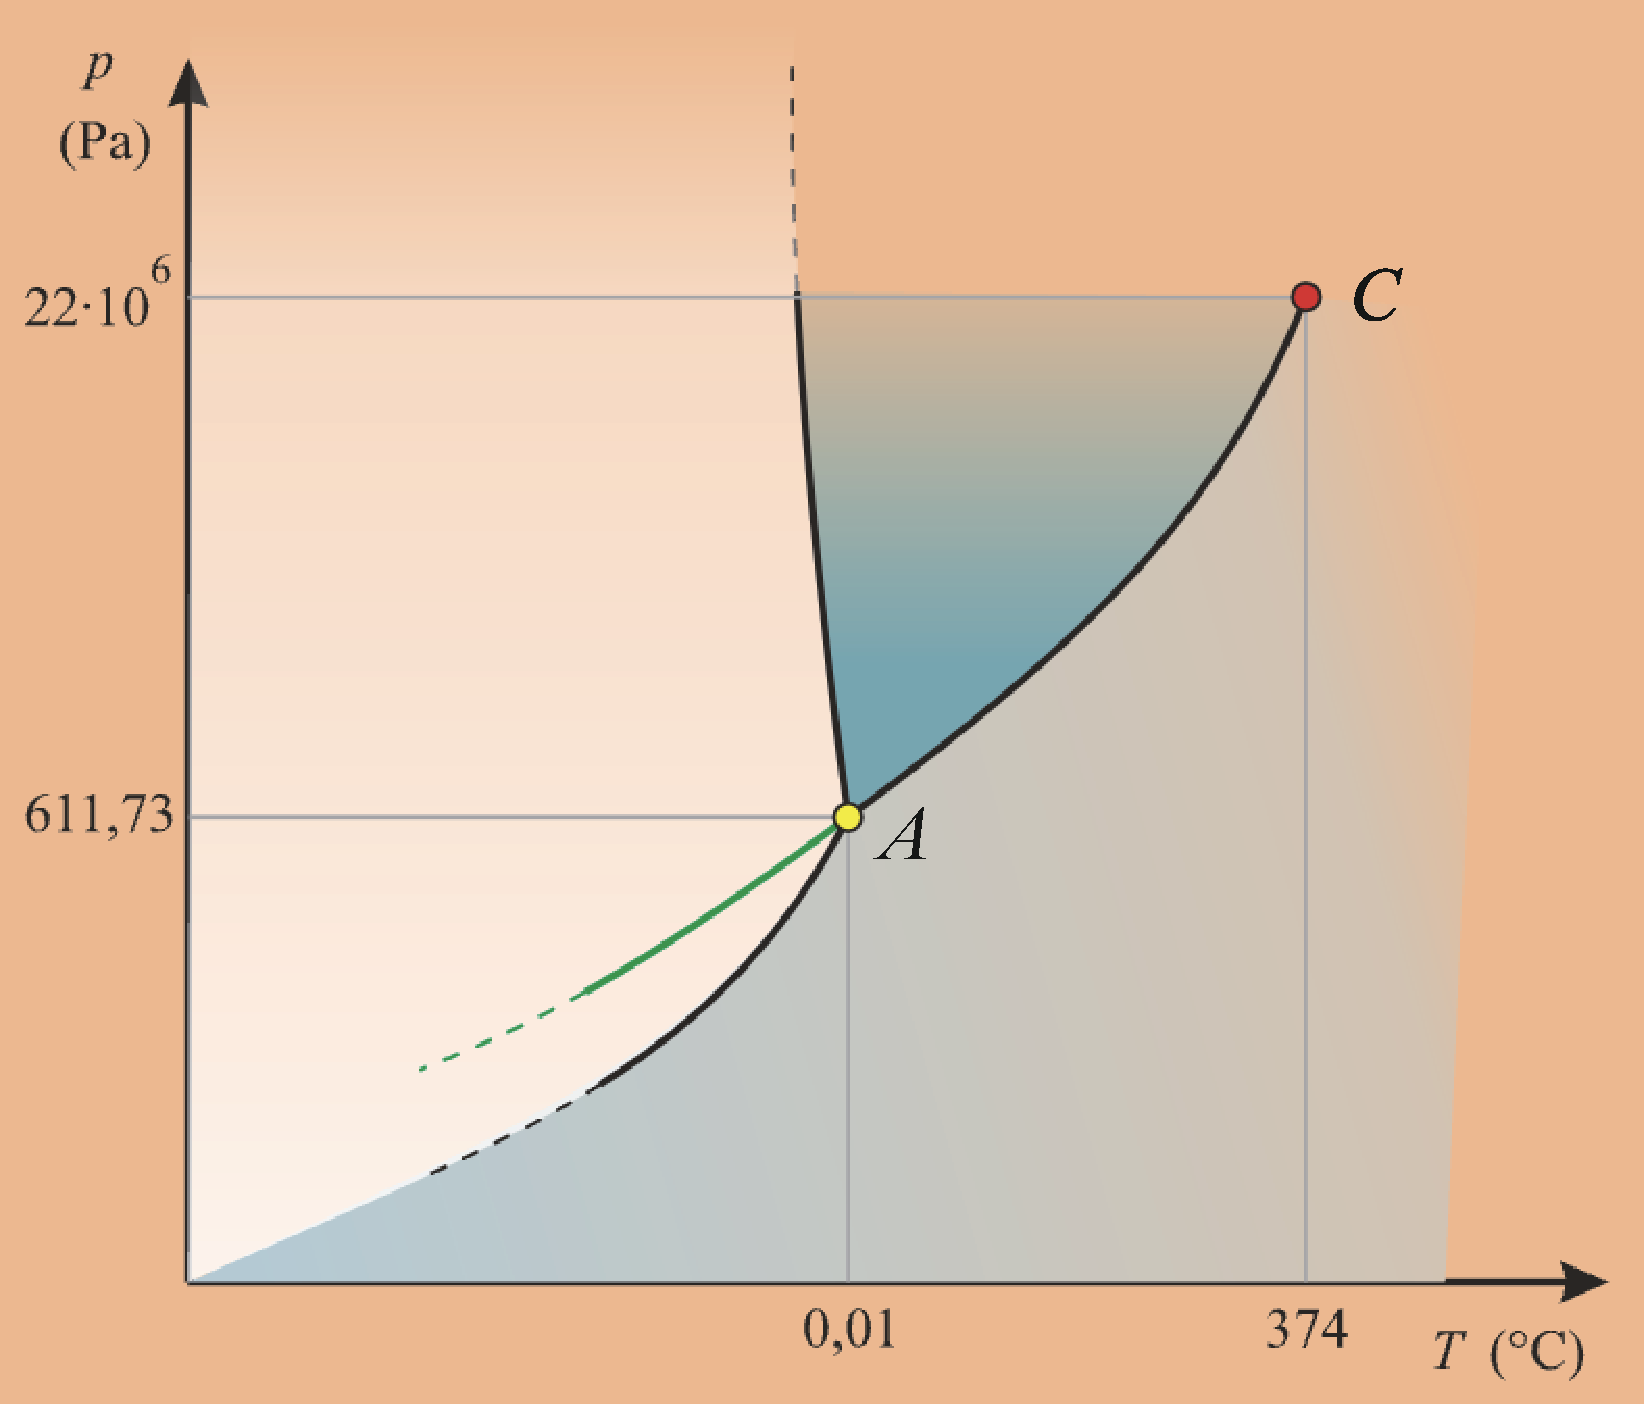
\includegraphics[width=0.5\linewidth]{images/thermal-21}
	\caption{水的相图,注意其中的三相点和临界点}
	\label{fig:thermal-21}
\end{figure}


在同样的$p-T$图像中还可以画出固、液两相能够共存的熔化曲线以及气、固相共存的升华曲线,合起来称为物质的\emph{相图}(phase diagram),图\ref{fig:thermal-21}给出的就是从实验中得到的水的相图。
在一个过程中系统穿过这些不同相的分界线时都会吸收或放出一定的热量,这个过程称为{\heiti 相变}(phase transition),这过程中交换的热量称为相变{\heiti 潜热}(latent heat)。
相图中有两个非常特殊的点需要引起注意,一个是气、液、固三相能够在一个唯一确定的温度和压强下共存,对应于图中的$A$点,称为物质的{\heiti 三相点}(triple point),今天我们就是用水的三相点来为绝对温度定标的。
另外和熔化线不同的是气化曲线并不是一条可以无限延伸的曲线,它从三相点出发最终终止于相图上的一点$C$,这一点上气体和液体的密度相等,已经没有任何方法能够对气液两相进行区分,称为{\heiti 临界点}(critical point)。




%%%%%%%%%%%%%
\begin{example}
	烧杯内盛有$0\si{\degreeCelsius}$的水,一块 0℃的冰浮在水面上,水面正好在杯口处.最后冰全部熔解成 0℃的水.在这过程中
	
	 A.无水溢出杯口,但最后水面下降了 
	 
	 B.有水溢出杯口,但最后水面仍在杯口处 
	 
	 C.无水溢出杯口,水面始终在杯口处 
	 
	 D.有水溢出杯口,但最后水面低于杯口
	\tagged{student}{\vspace*{0cm}}
	\begin{taggedblock}{teacher}
		
		解析:c
	\end{taggedblock}
\end{example}
%%%%%%%%%%%%%%%%%%%%


%%%%%%%%%%%%%
\begin{example}
	一杯水放在炉上加热烧开后,水面上方有“白色气”;夏天一块冰放在桌面上,冰的上方 也有“白色气”. 
	
	A.前者主要是由杯中水变来的“水的气态物质”
	
	B.前者主要是由杯中水变来的“水的液态物质”
	
	C.后者主要是由冰变来的“水的气态物质”
	
	 D.后者主要是由冰变来的“水的液态物质”
	\tagged{student}{\vspace*{4cm}}
	\begin{taggedblock}{teacher}
		
		解析:b
	\end{taggedblock}
\end{example}
%%%%%%%%%%%%%%%%%%%%

\begin{example}
已知水在100\si{\degreeCelsius}的饱和蒸气压 $p_0=101\si{kPa}$,在此温度、压力下水的摩尔相变潜热为$ 40.668\si{KJ/mol}$。 求在 100\si{\degreeCelsius},101\si{ kPa} 下使 1\si{ kg} 水蒸气全部凝结成液体水时的内能变化量。(忽略液态水的体积)
\tagged{student}{\vspace*{2cm}}
\begin{taggedblock}{teacher}
\newline
解析:$\frac{1\si{kg}}{18\si{g}}*40.668\si{KJ/mol}=2259\si{KJ}$
\end{taggedblock}
\end{example}

%%%%%%%%%%%%%
\begin{example}
	一端封闭的均匀管子,内有空气和水银蒸汽,被 10cm长的水银柱封闭 (不论管子如何放) . 当管子水平放置时, 这空气柱稳定长为17cm, 管子竖直放置时, 空气稳定柱长为20 cm , 如果大气压强为76 cmHg, 求水银蒸汽饱和蒸汽压.
	\tagged{student}{\vspace*{4cm}}
	\begin{taggedblock}{teacher}
		\newline
		解析:$(76+10-p_0)*17=(76-p_0)*20$   解出$p_0=19.3cmHg$
	\end{taggedblock}
\end{example}
%%%%%%%%%%%%%%%%%%%%



%%%%%%%%%%%%%
\begin{example}
	一汽缸的初始体积为$V$,其中盛有 2 \si{mol} 的空气和少量的水(水的体积可以忽略)。平衡时气体的总压强是 3.0 atm,经做等温膨胀后使其体积变为$ 2V$,在膨胀结束时,其中的水刚好全部消失,此时的总压 强为 2.0 atm。试计算此时:
	\\1.汽缸中气体的温度; 
	\\2. 若让其继续作等温压缩,使体积变为$ V/2$,汽缸中气体的总压强。 
	\\3. 若让其继续作等温膨胀,使体积变为$ 4V$,汽缸中气体的总压强。
	\tagged{student}{\vspace*{4cm}}
	\begin{taggedblock}{teacher}
		\newline
		解析:1.气体温度未改变,饱和蒸气压为1atm,气温为373K.
		\\2.压缩为$\frac{V}{2}$后,水蒸气为1atm,空气压为4atm,合起来是5atm
		\\3.在膨胀过程中,混合气体可按理想气体处理,压强变为1atm
	\end{taggedblock}
\end{example}
%%%%%%%%%%%%%%%%%%%%

\begin{example}
正确使用压力锅的方法是:将己盖好密封锅盖的压力锅加热,当锅内水沸腾时再加盖压力阀 S, 此时可以认为锅内只有水的饱和蒸气,空气己全部排除.
然后继续加热,直到压力阀被锅内的水蒸气顶起时,锅内即已达到预期温度(即设计时希望达到的温度),现有一压力锅,正确加热能达到的预期温度为 120\si{\degreeCelsius},大气压为\num{1.01e5}\si{Pa}。

若未按正确方法使用压力锅,在点火前就加上压力阀。此时锅内温度为10\si{\degreeCelsius},那么加热到压力阀刚被顶起时,锅内水的温度是多少?若继续加热,锅内水的温度最高可达多少?假设空气不溶于水.已知:水的饱和蒸气压$p_W(t)$与摄氏温度的关系图线如下图所示。
\begin{center}
	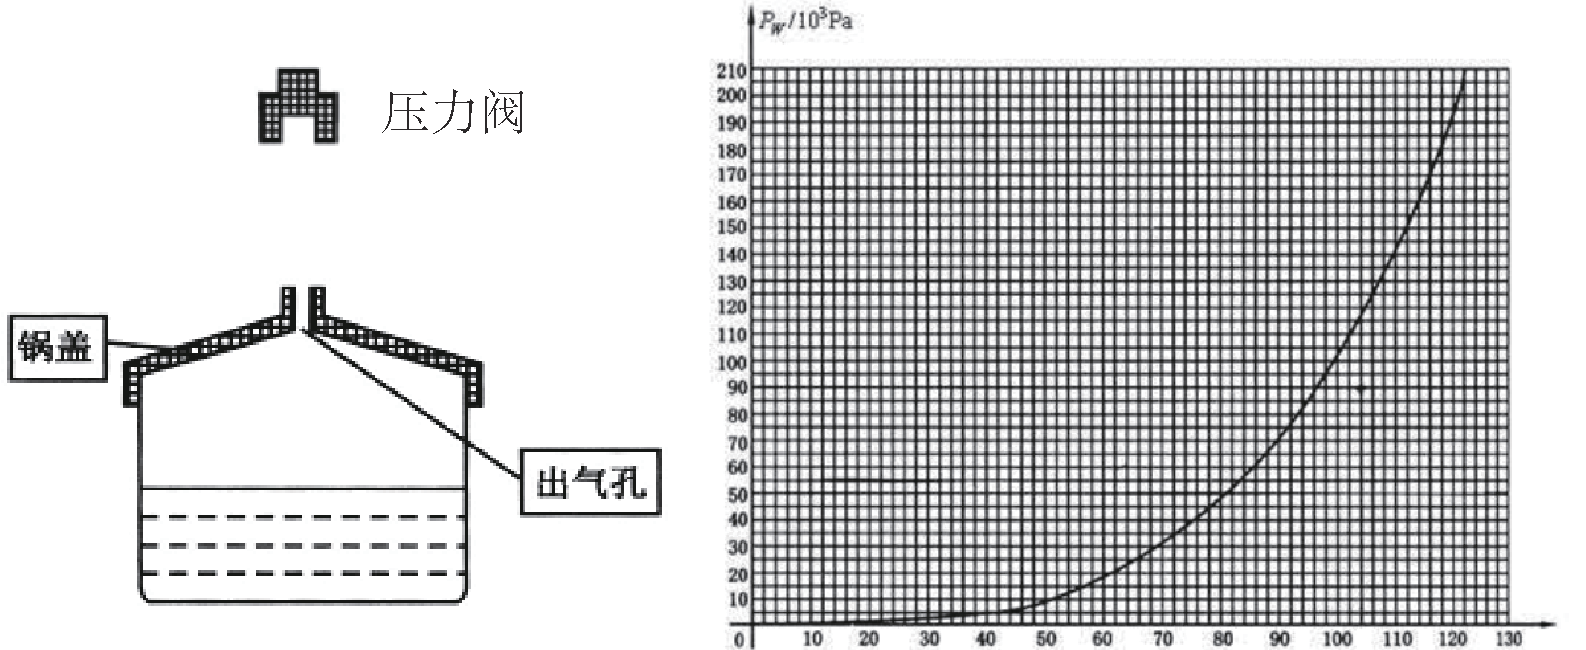
\includegraphics[width=0.95\textwidth]{images/thermal-18.pdf}
\end{center}
\tagged{student}{\vspace*{4cm}}
\begin{taggedblock}{teacher}
\noindent
解析:1.$p=291-\frac{t+273}{273}*101$ 画图,与图2交于一点,大概温度为$112\si{\degreeCelsius}$
\\2.最高可达$120\si{\degreeCelsius}$,把里面的空气都排走了
\end{taggedblock}
\end{example}


\begin{example}
以下是一个形成云的简单模型。
热空气与带着地球表面水蒸气的上升,当升到一定高度时气体压强降低到水蒸气的饱和蒸气压,水气开始凝结成水结,云就产生了。
假设空气是一种由氢和氧构成的理想气体,它们的比例为21:79。
令$g$为重力加速度,忽略它随高度的变化,气体上升过程中可以近似地认为是绝热过程。
在这些假设下可以证明压强随温度的变化满足
\[
p=p_0\left(\frac{T_0-\Gamma z}{T_0}\right)^\alpha
\]
这里$p_0$和$T_0$分别是海平面($z=0$)处的压强和温度,$\Gamma>0$为地球温度随高度的变化率。

(a)用已知物理量$\gamma$,$R$,$g$和$m_a$给出$\Gamma$的表达示,其中$\gamma$为绝热系数,$m_a$为摩尔质量。

(b)试估计高度升高\SI{1}{km}时温度的改变量。

(c)压强会随高度的升高而降低,试将压强随温度关系式中的$\alpha$用$\gamma$表示出来。

(d)在该模型当中大气层的总厚度为多少?

(e)饱和蒸气压随温度的变化由
\[
\frac{dp_s}{dT}=\frac{L}{T(v_2-v_1)}
\]
其中$L$是相变潜势,$v_{1,2}$是两相之间的体积差。
试在$v_2\ll v_1$的极限下求出饱和蒸气压与温度的关系。


(f)找出水蒸气开始凝结的条件。


\tagged{student}{\vspace*{9cm}}
\begin{taggedblock}{teacher}
\noindent
解析:国际竞赛题
\end{taggedblock}
\end{example}




\section{热传递}
热量的吸收与发射有三种方式:{\heiti 热辐射}(radiation),{\heiti 热对流}(convection)与{\heiti 热传递}(conduction)。当相互接触的两个物体温度不同时,我们知道热量会由高温物体传向低温物体,这个过程被称为热传递。
一个显著特点是热传递并不是瞬时发生的,无论是趋于平衡的过程还是持续的热传递都需要一定的时间。
不同物体的导热性质有着很大的不同,例如金属导热就远比棉花要快得多。
单位时间里通过某一介质或表面传递的热量依赖于导热介质的性质、形状、温差或其它因素。

设想在两个恒温的热源$T_1$和$T_2$之间仅由一个柱形导热介质相连接,其余部分均为绝热。
当达到稳定状态以后单位时间里由高温热源传向低温热源的热量满足{\heiti 傅里叶热传递定律}(Fourier's Law of Heat Conduction)
\begin{equation}
\Delta q = \kappa \frac{S}{L}(T_1-T_2)
\end{equation}
式中$S$为导热介质的横截面积、$L$为其长度,$\kappa$为一比例系数,称为导热介质的{\heiti 热导率}(conductivity),由介质的微观性质决定,单位是瓦特/米 $\cdot$ 开尔文(W/m $\cdot$ K)。
对于直接接触、当中无介质的两个物体之间的传热过程,例如放在空气当中的高温物体,这时热传递只正比于它们的温度差、接触的表面积和两个物体之间热传递性质:
\begin{equation}
\Delta q = k S (T_1-T_2),
\end{equation}
在处理热传递问题中要注意这两种情况的不同。

稳定热传递状态的热平衡状态有所不同,达到热平衡状态的系统各部分之间有着相同的温度,稳定的热传递状态则不同,系统各部分之间的温度虽然有所不同,但对于系统内部任意的闭合区域来说,如果相同时间里流入的热量都等于流出的热量时,这部分区域内就没有热量的净流入或流出,它的温度不会发生变化。
根据稳定条件以及热传递的性质就可以决定处于稳定热传递系统内部各点的温度。
\begin{example}
试证明稳定热传导状态下处于两个大热源之间柱形均匀传热介质上的温度分布必为线性分布。
即建立如图所示的坐标系,杆的温度与坐标$x$的函数为\[T(x)=T_1+(T_2-T_1)\frac{x}{L}.\]
\tagged{student}{\vspace*{4cm}}
\begin{taggedblock}{teacher}
\newline
解析:略
\end{taggedblock}
\end{example}







\begin{example}
一厚度为$t$的薄金属盘悬吊在温度为 $300\unit{K}$的空气中,其上表面受太阳直射,温度为$360\unit{K}$,下表面温度为$340\unit{K}$。
空气的温度保持不变,单位时间内金属盘每个表面散失到空气中的能量与此表面和空气的温度差以及此表面的面积成正比,忽略金属盘侧而的能量损失。
若金属盘的厚度变为原来的2倍,求金属盘上、下表面的温度。
\tagged{student}{\vspace*{4cm}}
\begin{taggedblock}{teacher}
\newline
解析:$333.3\si{K},366.7\si{K}$
\end{taggedblock}
\end{example}

%%%%%%%%%%%%%
\begin{example}
	温度开关用厚度均为0.20~\si{mm}的钢片和青铜片作感温元件;在温度为$20^\circ C$时,将它们紧贴,两端焊接在一起,成为等长的平直双金属片。
	若钢和青铜的线膨胀系数分别为\num{1.0e-5}\si{/K}和\num{1.0e-5}\si{/K}
	当温度升高到$120^\circ C$时,双金属片将自动弯成圆弧形,如图所示。
	试求双金属片弯曲的曲率半径。 (忽略加热时金属片厚度的变化)
	\tagged{student}{\vspace*{4cm}}
	\begin{taggedblock}{teacher}
		\newline
		解析:$r=\frac{2+(\alpha_1+\alpha_2)(T_2-T_1)}{2(\alpha_2-\alpha_1)(T_2-T_1)d}=2.0*10^2\si{mm}$
	\end{taggedblock}
\end{example}
%%%%%%%%%%%%%%%%%%%%

